\documentclass{article}
\usepackage{iclr2027_conference,times}
\input{math_commands.tex}
\usepackage{hyperref}
\usepackage{url}
\usepackage{amsmath,amssymb,amsthm}
\usepackage{booktabs}
\usepackage{graphicx}
\usepackage{tikz}
\usetikzlibrary{calc,arrows.meta,positioning}
\usepackage{pgfplots}
\pgfplotsset{compat=1.18}

\providecommand{\cW}{\mathcal{W}}
\providecommand{\cA}{\mathcal{A}}
\providecommand{\cS}{\mathcal{S}}
\providecommand{\cN}{\mathcal{N}}
\providecommand{\ba}{\mathbf{a}}
\newcommand{\smr}{\textsc{SMR}}
\newcommand{\simthree}{\mathrm{Sim}(3)}
\newcommand{\gvec}{\mathbf{g}}
\newcommand{\hvec}{\mathbf{h}}
\newtheorem{proposition}{Proposition}

\title{Give Geometry Models a Real Memory:\\A Neural Scaffold for Frozen 3D Foundation Models}

\author{Anonymous authors\\ \texttt{under double-blind review}}

\iclrfinalcopy
\begin{document}
\maketitle

\begin{abstract}
Geometry foundation models are superb eyes attached to no memory. Within
one forward pass they recover cameras and dense structure; past it, their
estimates are glued across windows, and every glue joint leaks. Streaming
variants move the memory into the weights---a cache of past tokens---but a
cache cannot \emph{correct}: it cannot revise a pose once emitted, cannot
verify that a familiar-looking place is the same place, and does not
outlive the sequence. We identify the missing organ as an
\emph{error-correcting memory} and build one. \smr{} adapts the grid-cell
scaffold of Vector-HaSH to metric vision: the backbone's reference poses
clamp activity bumps on head-direction attractor rings, bump velocities
drive spatial grid modules, and the concatenated field activities form a
grid code that indexes a bank of the backbone's own outputs, bound one-shot
through fixed random projections and plastic associative weights. The
scaffold's dynamics correct one class of error for free---states consistent
with no location---and are, by construction, blind to the other: coherent
drift, which describes a legitimate somewhere else. That blind class is
exactly what geometry can fix: recognized revisits are re-measured by the
backbone itself in one anchored pass, accepted only on two-site consensus,
and used to re-clamp the past. The memory is gradient-free, adds a
guaranteed floor (bit-identical to the backbone within one window), and one
implementation serves six frozen and two streaming backbones. It recovers
most of the accuracy lost to window seams at $200$ frames (VGGT
$90.0\!\to\!93.7$ AUC@30 on CO3Dv2), improves a single pass from within by
reading repeated writes (DTU $0.441\!\to\!0.396$\,mm, better on every
scan; novel views through a fixed rendering head ${+}0.24$\,dB), restores the
$200$-frame regime to streaming models whose native
memory cannot allocate it, and turns a frozen backbone into a training-free
SLAM system with the best average error on 7-Scenes ($0.029$\,m on seq-01,
$0.038$ on the full test split).
\end{abstract}

\section{Introduction}
\label{sec:intro}
% Figure 1: system overview (TikZ, compiles with the paper; no external assets).
\begin{figure}[t]
\centering
\resizebox{\textwidth}{!}{%
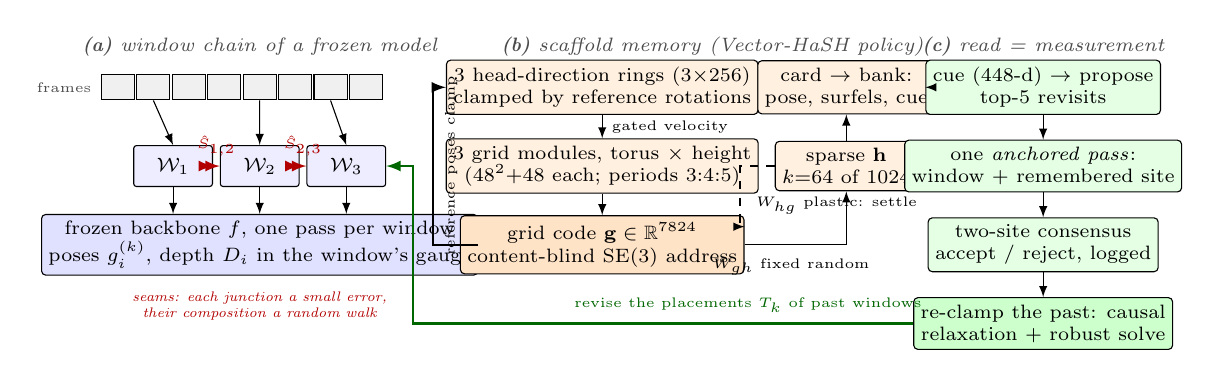
\begin{tikzpicture}[
  font=\scriptsize, >=latex,
  box/.style={draw, rounded corners=1.5pt, align=center, inner sep=2.5pt, minimum height=5.2mm},
  frame/.style={draw, fill=gray!12, minimum width=4.2mm, minimum height=3.2mm, inner sep=0pt},
  win/.style={draw, rounded corners=1pt, fill=blue!7, minimum width=10mm, minimum height=5.2mm, align=center, inner sep=1.5pt},
  mem/.style={draw, rounded corners=1.5pt, fill=orange!12, align=center, inner sep=2.5pt, minimum height=5.6mm},
  read/.style={draw, rounded corners=1.5pt, fill=green!10, align=center, inner sep=2.5pt, minimum height=5.6mm},
  lbl/.style={font=\scriptsize\itshape, text=black!70}]
% ---------------- (a) frozen backbone on windows, glued by Sim(3) ----------------
\foreach \i in {0,...,7} { \node[frame] (f\i) at (0.45*\i, 0.15) {}; }
\node[lbl, anchor=east, font=\tiny] at (f0.west) {frames};
\node[win] (w1) at (0.7, -0.85) {$\cW_1$};
\node[win] (w2) at (1.8, -0.85) {$\cW_2$};
\node[win] (w3) at (2.9, -0.85) {$\cW_3$};
\draw[->] (f1.south) -- (w1.north); \draw[->] (f4.south) -- (w2.north); \draw[->] (f6.south) -- (w3.north);
\node[box, fill=blue!12, minimum width=34mm] (bb) at (1.8, -1.85) {frozen backbone $f$, one pass per window\\ poses $g_i^{(k)}$, depth $D_i$ in the window's gauge};
\draw[->] (w1.south) -- (w1.south |- bb.north); \draw[->] (w2.south) -- (w2.south |- bb.north); \draw[->] (w3.south) -- (w3.south |- bb.north);
\draw[<->, red!70!black, thick] (w1.east) -- node[above, font=\tiny, text=red!70!black] {$\hat S_{1,2}$} (w2.west);
\draw[<->, red!70!black, thick] (w2.east) -- node[above, font=\tiny, text=red!70!black] {$\hat S_{2,3}$} (w3.west);
\node[lbl, text=red!70!black, anchor=north, font=\tiny\itshape, align=center] at (1.8, -2.32) {seams: each junction a small error,\\ their composition a random walk};
% ---------------- (b) scaffold memory ----------------
\node[mem, minimum width=25mm] (rings) at (6.15, 0.15) {3 head-direction rings ($3{\times}256$)\\ clamped by reference rotations};
\node[mem, minimum width=25mm] (mods) at (6.15, -0.85) {3 grid modules, torus $\times$ height\\ ($48^2{+}48$ each; periods $3{:}4{:}5$)};
\node[mem, minimum width=25mm, fill=orange!22] (code) at (6.15, -1.85) {grid code $\gvec\in\mathbb R^{7824}$\\ content-blind $\mathrm{SE}(3)$ address};
\draw[->] (rings) -- node[right, font=\tiny] {gated velocity} (mods);
\draw[->] (mods) -- (code);
\node[mem, minimum width=17mm] (h) at (9.25, -0.85) {sparse $\hvec$\\ $k{=}64$ of $1024$};
\node[mem, minimum width=17mm] (card) at (9.25, 0.15) {card $\to$ bank:\\ pose, surfels, cue};
\draw[->] (code.east) -- (9.25,-1.85) -- (h.south);
\node[font=\tiny, anchor=north] at (8.55,-1.9) {$W_{gh}$ fixed random};
\draw[->, dashed] (h.west) -- (7.9,-0.85) -- (7.9,-1.62) -- (code.east |- 0,-1.62);
\node[font=\tiny, anchor=west] at (7.98,-1.35) {$W_{hg}$ plastic: settle};
\draw[->] (h) -- (card);
\draw[->, thick] (bb.east) -- (4.0,-1.85) -- (4.0,0.15) -- (rings.west);
\node[font=\tiny, rotate=90, anchor=north] at (4.03,-0.85) {reference poses clamp};
% ---------------- (c) the read is a measurement ----------------
\node[read, minimum width=22mm] (cue) at (11.75, 0.15) {cue ($448$-d) $\to$ propose\\ top-5 revisits};
\node[read, minimum width=22mm] (anch) at (11.75, -0.85) {one \emph{anchored pass}:\\ window $+$ remembered site};
\node[read, minimum width=22mm] (cons) at (11.75, -1.85) {two-site consensus\\ accept / reject, logged};
\node[read, fill=green!20, minimum width=22mm] (pgo) at (11.75, -2.85) {re-clamp the past: causal\\ relaxation $+$ robust solve};
\draw[->] (card.east) -- (cue.west);
\draw[->] (cue) -- (anch); \draw[->] (anch) -- (cons); \draw[->] (cons) -- (pgo);
\draw[->, thick, green!40!black] (pgo.west) -- (3.75,-2.85) -- (3.75,-0.85) -- (w3.east);
\node[font=\tiny, text=green!40!black, anchor=south] at (8.0,-2.83) {revise the placements $T_k$ of past windows};
% panel labels
\node[lbl, anchor=south] at (1.8, 0.42) {\textbf{(a)} window chain of a frozen model};
\node[lbl, anchor=south] at (7.55, 0.42) {\textbf{(b)} scaffold memory (Vector-HaSH policy)};
\node[lbl, anchor=south] at (11.75, 0.42) {\textbf{(c)} read = measurement};
\end{tikzpicture}}
\vspace{-3mm}
\caption{\textbf{\smr{} at a glance.} (a) Beyond its window a frozen geometry model is a chain of Sim(3)
junctions; every seam leaks and cross-window pairs inherit the walk. (b) The backbone's reference poses
clamp head-direction rings; bump velocities drive grid modules; the concatenated field activities are a
content-blind grid code that indexes cards (pose, surfels, cue) through a fixed random projection and a
plastic return map, which settles incoherent states and is blind to coherent shifts (Prop.~\ref{prop:coherent}).
(c) A recalled place is a hypothesis: it is re-measured by the backbone itself in one anchored pass, accepted
only on two-site consensus, and used to re-clamp the past. Within one window nothing changes: the system
is bit-identical to the backbone.}
\label{fig:system}
\end{figure}

Ask VGGT \citep{vggt} for the relative pose of two frames inside one window
and you get the judgment of a foundation model. Ask it for two frames ten
seconds apart and you are no longer asking the model at all---you are asking
a chain of glue joints. Beyond its context window, every feed-forward
geometry model \citep{vggt,vggtomega,pi3,dust3r,mast3r,fast3r} is deployed
the same way: run on overlapping windows, each window's output in its own
gauge with its own scale, consecutive windows aligned by a similarity fitted
on a few shared frames (Fig.~\ref{fig:system}a). Each junction is nearly
right. Composed, they are a random walk \citep{strasdat}: the error between
frames $m$ windows apart grows with $m$, and the pairs that dominate any
long-input metric are precisely the pairs assembled through the most joints.
The model never became less accurate; the \emph{system around it} has no way
to notice that frame 190 shows the same hydrant as frame 5, and no way to
use that fact.

Streaming models answer by training memory into the weights: CUT3R's
recurrent state, StreamVGGT's and STream3R's causal token caches
\citep{cut3r,streamvggt,stream3r}. This extends the horizon, and within it
these models are strong. But a cache is memory without an eraser. It cannot
\emph{revise}: poses already emitted are final, so the defining act of loop
closure---correcting the past upon return---does not exist. It cannot
\emph{verify}: attention is soft, so a look-alike corridor contaminates the
state silently, leaving no residual and no record. It does not
\emph{persist}: the cache grows with the sequence, dies with the process, and
leaves nothing to localize against tomorrow. Window models and streaming
models bleed from the same wound at different rates: \textbf{errors, once
made, have nowhere to be corrected from.}

Naming the wound specifies the cure. An error-correcting memory for geometry
must (i)~\emph{recognize} that the present overlaps the past;
(ii)~\emph{re-measure} rather than assume---recognition is fallible;
(iii)~\emph{revise} estimates already made; (iv)~\emph{persist} across
sequences and scenes; and (v)~\emph{never touch} what the model already does
well inside its window. Classical SLAM built such memories for classical
pipelines \citep{grisetti,elasticfusion}, but its instruments assume
calibrated features and consistent scale; the outputs of frozen geometry
models are gauge-free, scale-drifting, and covariance-less, and in our
development every attempt to strengthen alignment with their dense
predictions made accuracy \emph{worse} (App.~\ref{app:fusion}). The one
trustworthy instrument left is the backbone itself.

\smr{} is that memory (Fig.~\ref{fig:system}). Its skeleton comes from the
hippocampus by way of Vector-HaSH \citep{vectorhash}: content is stored not
by associating patterns with patterns but by binding it to states of a
prestructured \emph{scaffold} of grid-cell modules, whose combinatorial state
space carries the capacity. We make the scaffold metric and real: the
backbone's reference poses clamp activity bumps on head-direction attractor
rings; the bumps' motion drives spatial grid modules; the concatenated field
activities form the grid code that addresses a bank holding the backbone's
own poses, surfels, and appearance (Sec.~\ref{sec:scaffold}). The scaffold's
associative loop \emph{settles} away any state inconsistent with being
somewhere---and is blind to coherent drift, the state consistent with being
somewhere \emph{else} (Prop.~\ref{prop:coherent}). That blindness is the
design's hinge, not its flaw: the blind class is exactly what geometry can
fix, by re-measuring recognized revisits with the backbone in a single
anchored pass, accepting only two-site consensus, and re-clamping the past
(Sec.~\ref{sec:read}). Dynamics and geometry divide the labor of error
correction between them.

\textbf{Contributions.} \textbf{(1)} A diagnosis: window and streaming
geometry models fail long inputs for one shared reason, the absence of an
error-correcting memory, from which five requirements follow.
\textbf{(2)} The first transfer of grid-cell scaffold memory to metric 3D
perception with the dynamics kept: real attractor fields, one-shot binding of
a frozen model's outputs, capacity in the scaffold, and a division-of-labor
principle---settle the incoherent, pin the coherent---stated as a
proposition. \textbf{(3)} A verified geometric read--write loop (recognize,
re-measure with the backbone itself, two-site consensus, re-clamp) with a
guaranteed floor: within one window the system is bit-identical to the bare
backbone, so the backbones' own benchmarks become our controls.
\textbf{(4)} Breadth as evidence: one implementation and one hyperparameter
set over six frozen and two streaming backbones, evaluated on camera pose
versus input length, dense MVS and point maps, SLAM, and novel view
synthesis, with every negative cell retained.

\section{Where geometry models bleed, and why existing memories do not stop it}
\label{sec:bleed}
\textbf{Window models: seams.} A frozen backbone $f$ maps $W$ images to
per-frame cameras and depth $(g_i,D_i)$ in the gauge of the window's first
frame \citep{vggt}. A long sequence is covered by windows
$\cW_1,\dots,\cW_K$ ($W{=}32$, overlap $O{=}16$ throughout), and consecutive
windows are glued by the similarity---rotation, translation, \emph{and
scale}---that best maps shared-frame poses onto each other:
\begin{equation}
\label{eq:junction}
\hat S_{k,k+1}=\argmin_{S\in\simthree}
\sum_{j\in\cW_k\cap\,\cW_{k+1}}\rho\big(d(S\cdot g_j^{(k+1)},\,g_j^{(k)})\big),
\end{equation}
solved closed-form \citep{umeyama,horn} inside a robust loop with a scale
gate (App.~\ref{app:sim3}). Every $\hat S$ carries a small error; their
composition is a walk whose variance grows along the chain. Split a long-input pairwise metric by pair type and the bleed localizes:
\emph{within-window} pairs are the backbone's own judgment; \emph{cross-window}
pairs inherit the walk and are $O(1{-}W/N)$ of all pairs at $N$ frames.
Long-input accuracy is decided by the pairs no forward pass ever judged.

\textbf{Streaming models: write-once memory, paid for in VRAM.} Causal
models fold the past into a state the present attends to
\citep{cut3r,streamvggt,stream3r}. The state helps the \emph{next}
prediction; it cannot help the previous one. On revisit the model may
perceive the return, but its history of emitted poses stays bent; no
mechanism lets new evidence flow backward, no gate separates genuine from
apparent familiarity, and nothing survives the end of the stream. These are
not training deficiencies; they are absent operations. The implicit memory
also has a price that grows with the sequence: StreamVGGT's token cache grows
linearly with input length and STream3R's causal attention mask
quadratically. On a 46\,GB GPU we measure the walls (Fig.~\ref{fig:results}c,
App.~\ref{app:compute}): StreamVGGT completes $100$-frame sequences and
exhausts memory at $200$; STream3R's mask allocation alone requests
${\sim}9$\,GB beyond capacity at $50$ CO3D frames and $281$\,GB at $200$.
The wall is not peculiar to streaming (single-pass $\pi^3$ exhausts the same
GPU at $200$ frames), so windowing at scale is a necessity for every
architecture; the open question is whether it must cost accuracy.

\textbf{What classical and biological memory offer.} Loop-closure
detection, pose graphs, and surfel maps are the spine of classical SLAM
\citep{grisetti,strasdat,elasticfusion}, and recent systems put
foundation-model front ends on that spine
\citep{mast3rslam,vggtslam,vistaslam,slamformer}; their instruments still
assume a consistent measurement channel, which frozen geometry models do not
provide, so the measurement role must pass to the backbone itself. For the
memory's \emph{organization} we turn to Vector-HaSH \citep{vectorhash}:
binding content to a prestructured grid-cell scaffold yields high-capacity,
robust episodic memory, and \smr{} is, to our knowledge, its first transfer
to metric perception---dynamics retained, cleanup kept where it is competent,
geometric verification added where it is blind (related work:
App.~\ref{app:related}).

\section{\smr{}: a scaffold memory that corrects errors}
\label{sec:method}

\subsection{From reference poses to a grid code}
\label{sec:scaffold}
The memory's state is not a buffer but a small dynamical system, built from
Amari-type neural fields with genuine bump dynamics and updated in time. The
flow runs from the backbone's poses to a single code (Fig.~\ref{fig:system}b).

\emph{Orientation first.} Each input view's reference pose (the backbone's
output, made global by the current window placement) clamps activity bumps
on three \emph{head-direction rings} of $256$ units (ZYX Euler). Between
clamps, rotational velocity moves the bumps through the gate
$R(\hat\psi,\hat\theta,\hat\phi)$---the unique gating under which ring-phase
increments are exact differentials of camera rotation, so integrating them
is path-independent (measured $9.3\times$ accuracy gap over alternative
gatings; App.~\ref{app:vhash}).

\emph{Position through the modules.} The bumps' translational velocity,
rotated into the world frame by the ring readout, drives three \emph{spatial
grid modules}. Each module is a $48{\times}48$ torus (horizontal phase) plus
a $48$-unit ring (height), with spatial periods $\{2.4,3.2,4.0\}$ in
normalized scene units---the smallest coprime ladder $3{:}4{:}5$, whose joint
phase is unambiguous over a Chinese-remainder range of
$2.4\cdot\mathrm{lcm}(3,4,5)=144$ units, beyond any benchmark scene; adding a
module multiplies the range, so capacity in extent is additive hardware, not
retuning.

\emph{The code.} Concatenating all field activities---three toruses, three
height rings, three head-direction rings---yields the grid code
$\gvec\in\mathbb R^{7{,}824}$. It is \emph{content-blind} (its axes are
$\mathrm{SE}(3)$ axes, so it can index anything) and \emph{placed, not
integrated}: every view clamps the state at a backbone pose, so the classical
failure of path-integration memories---drift from noisy velocity---is absent
by construction in the binding regime.

\subsection{The Vector-HaSH policy: scaffold, random projection, plastic return}
\label{sec:policy}
Capacity comes from the scaffold's state space, not from content--content
association. Following Vector-HaSH, the grid code is projected through a
\emph{fixed random} matrix to a sparse layer and returned through
\emph{plastic associative} weights,
\begin{equation}
\hvec=\sigma_k(W_{gh}\,\gvec),\qquad
\hat\gvec=\psi(W_{hg}\,\hvec),
\end{equation}
with $\sigma_k$ a top-$k$ threshold ($N_h{=}1024$, $k{=}64$) and $\psi$
per-field normalization. $W_{gh}$ is never trained; $W_{hg}$ is the memory's
plasticity---a Hebbian sum in Vector-HaSH's binary setting and, for our
continuous field templates (where the Hebbian sum is measurably at chance),
its continuous analogue: a ridge-regularized least-squares association formed
once from the scaffold's own states (App.~\ref{app:vhash}). Formation visits
states covering every module phase at spacing $\le\lambda_{\min}/6$; after
it, every joint phase is a fixed point of the loop.

The loop's power is selective, and the selectivity organizes the whole
system. Perturb $\gvec$ and decompose the perturbation: the \emph{incoherent}
part---module states that agree with \emph{no} location---is erased by
settling through the loop, continuously and for free. The \emph{coherent}
part---a shift describing some \emph{other} legitimate location---survives
settling untouched, because to every internal check it is a perfectly valid
state.
\begin{proposition}[Division of labor]
\label{prop:coherent}
After formation, every joint phase is a fixed point of the loop
$\gvec\mapsto\psi(W_{hg}\sigma_k(W_{gh}\gvec))$. A perturbation of a stored
state decomposes into a coherent component, which lands on another fixed
point and is therefore invariant under settling, and an incoherent
component, which is not a fixed point and is contracted by settling. No
internal dynamics can detect the coherent component; it can be corrected
only by an external clamp. (Argument in App.~\ref{app:vhash}.)
\end{proposition}
\smr{} pins the coherent part twice: continuously, by clamping at every
backbone pose; and retrospectively, by the verified closures of
Sec.~\ref{sec:read}.

\subsection{Cards, not photocopies: what gets bound}
\label{sec:content}
Each bound state associates the grid code with a \emph{card}: a compact
appearance cue plus an index into a bank where the heavy content lives---the
owning window, the frame's pose in the owner's gauge, its surfels (the
backbone's points with color and footprint \citep{surfels,elasticfusion}),
and per-primitive appearance. The card indirection lets one scaffold serve
arbitrarily heavy content at fixed loop cost, and per-module remap offsets
let many scenes coexist in one memory. Binding is one-shot and
gradient-free, gated by a bind-time novelty test calibrated against the
similarity floor of unrelated views (App.~\ref{app:cue}). The scaffold is content-addressable---an
appearance descriptor cues an address and the address returns the stored
views---so the same frozen descriptor keys and cues it. Which descriptor
depends on what the memory is asked to recognise. For revisits across a
scene it is a self-supervised global descriptor \citep{dinov2}, because
recognising a place from a new viewpoint is what such descriptors are trained
for; the $448$-dimensional engineered cue of App.~\ref{app:cue} keys the
rendering-recall memory instead, where the cue must be computable from a raw
frame before any backbone pass and identical across backbones. Keying on the
backbone's own features is the natural alternative and is measured, not
assumed (App.~\ref{app:ablations}): it ties the bank to one backbone, and a
plug-in memory must outlive its backbone.

\subsection{The read is a measurement: recognize, re-measure, verify}
\label{sec:read}
A remembered place is a hypothesis, not a constraint. When a new window's
frames cue the memory and a match older than the revisit gap returns,
\smr{} converts the proposal into geometry using the only instrument it
trusts: one \emph{anchored pass} of the backbone over the current window
plus a small remembered \emph{site} (the matched frame and a temporal
partner). Old and new views now sit in a single forward pass, so their
relative geometry is the model's joint judgment---no seams in between. Two
robust fits of Eq.~\ref{eq:junction} compose the pass into a candidate
closure $\hat Z\in\simthree$ (App.~\ref{app:closure}). One measurement is
still not trusted: acceptance requires \emph{two independent sites} whose
implied placements agree within scene-scaled tolerances---independent errors
rarely agree---and every acceptance and rejection is logged with its
residuals. Retrieval itself is two-stage for the same reason (propose
top-$5$, verify geometrically), which in controlled tests turned $22/39$
correct recalls into $39/39$ (App.~\ref{app:cue}).

The same read applies \emph{inside} one window, where no revisit exists
but two content-level errors do: a pass depends on the ordering of its
frames, and its point maps carry a scale bias against its own cameras.
Writing $K$ orderings of the same views to the same scaffold coordinates,
re-measuring each pass's scale against the stored cards of the shared views
(symmetric, no pass privileged), and returning the per-pixel consensus is
the read exercised densely (Sec.~\ref{sec:mvs}).

\subsection{The write-back revises the past}
\label{sec:correct}
Junctions and accepted closures form a pose graph over window placements
$T_k\in\simthree$. Online, each closure triggers a causal relaxation that
spreads the implied correction over the intervening windows in
$O(\text{span})$: the trajectory behind the camera bends into
consistency---the operation no write-once memory can express. At sequence
end a single robust solve (Huber loss, explicit scale weighting, one
outlier-rejection round \citep{huber,grisetti}) polishes the graph;
empirically the causal rule captures most of the correction. Frames inherit
their owner's placement, $\hat g_j=T_{k(j)}\,g_j^{(k(j))}$, which yields the
\emph{floor}: within-window relative geometry is exactly the backbone's own;
an input that fits one window is bit-identical to the bare model; and at any
observed view the memory returns the backbone's output under an exact group
action (App.~\ref{app:invariant}). The backbones' single-window benchmarks
are therefore not competitors' turf but our control experiments.

\section{Evaluation design}
\label{sec:tasks}
One implementation and one hyperparameter set (App.~\ref{app:repro}) serve
every evaluation; the tasks differ only in which memory operation they
exercise, and each is reported for every backbone as raw, +\smr{} (the causal
memory) and +\smr{}+PGO (adding the final solve). \emph{Camera pose versus
input length} (Sec.~\ref{sec:results-pose}) is the direct test of
Sec.~\ref{sec:bleed}: rows coincide for $N\le W$ by the floor and separate
as seams and revisits accumulate, and a dataset without revisits is the
control. \emph{Dense MVS and point maps} (Sec.~\ref{sec:mvs}) exercise the
read inside one window, where pose-level memory is inert by construction and
only the content read can act. \emph{SLAM} (Sec.~\ref{sec:results-slam})
runs the streaming memory as an online system against dedicated pipelines,
including the persistence test no implicit memory can enter. \emph{Novel view
synthesis} (Sec.~\ref{sec:nvs}) asks whether corrected geometry renders
better through one shared, lightly trained head.

\section{Experiments}
\label{sec:experiments}

\subsection{Camera pose versus input length}
\label{sec:results-pose}
We evaluate under the pairwise-pose protocol of \citet{vggt}: $N$ frames of
a sequence are given, and AUC@30 \citep{relposepp,posediffusion} scores all
frame pairs by the maximum of relative-rotation and translation-direction
error. We extend the protocol along its one hidden axis,
$N\in\{10,50,100,200\}$, on CO3Dv2 ($37$ ground-truth-validated sequences;
frames spread over each full sequence at every $N$) and RealEstate10K (the
official test-1800 split at $N{=}10$, $1{,}653$ live clips; $100$ clips with
${\ge}200$ frames for the length axis). Table~\ref{tab:pose} reports every
cell; Fig.~\ref{fig:results} draws the curves.

% built 2026-09-05 07:17 by scripts/build_main_table.py from /tmp/mr3/outputs/reports/matrix
\begin{table}[t]
\centering\scriptsize
\setlength{\tabcolsep}{2.4pt}
\caption{Camera pose, dense MVS and point maps for every backbone, raw and with the memory.
\textbf{Camera pose} (AUC@30$\uparrow$ versus number of input frames $N$): raw = Sim(3)-chained
windows; +\smr{} = causal scaffold memory; +\smr{}+PGO adds the final robust solve. At $N{=}10$
(one window) and, on these data, $N{=}50$ (no revisits yet) the three rows are identical --- the
floor of Sec.~\ref{sec:correct}, measured. $^{\dagger}$DUSt3R/MASt3R length axis on a stated
10-sequence CO3D subset (pairwise-alignment runtime); their RE10K length cells are a 10-clip
subset$^{\ddagger}$. Native and $^{\ddagger}$ windowed cells at $N{=}10$ differ only by sample
(100 vs.\ 10 clips). OOM = exceeds a 46\,GB GPU. RE10K frames are uniform $\le$480p
re-extractions shared by all rows.
\textbf{Dense MVS} (DTU, 22 standard scans, all 49 views, Chamfer mm$\downarrow$) and
\textbf{point maps} (ETH3D, 13 scenes, ten frames, official rendered depth and masks,
Umeyama on per-pixel correspondences, Chamfer m$\downarrow$): one harness for every row.
Official DTU evaluator (masks, 0.2\,mm downsampling); gauge = Sim(3) refinement onto the scan,
chosen by a symmetric fit criterion among the camera alignment, a region-restricted
point-to-plane ICP, and the same from a robust similarity initialisation. Each backbone
contributes its native point map (point head where it has one, depth $\times$ camera
otherwise) with confidence $>2$ (top 68\% for sigmoid confidences). Both benchmarks fit one
window: raw is the single pass; +\smr{} is the memory's in-window read --- four orderings of the
same views written to one scaffold, symmetric re-measure of per-pass scale, consensus (median
on DTU, corroborated pixels only on ETH3D). No junction graph exists inside one window, so
+\smr{}+PGO equals +\smr{}. The read is the identity for order-invariant backbones (DUSt3R and
MASt3R: pairwise + global alignment; $\pi^3$: permutation-equivariant), and it presupposes
commensurable passes: for Fast3R and the causal StreamVGGT/STream3R, orderings yield
different reconstructions and the corroborated read keeps too little (ETH3D). DUSt3R on DTU
uses a sliding-window pair graph (window 5); its complete graph over 49 views exceeds 46\,GB.
$^{\S}$The VGGT-$\Omega$ authors report possible benchmark contamination of the released
checkpoint; ETH3D's training scenes are this benchmark. Streaming backbones: native = one causal
pass; windowed rows use 16-view windows fused by their median, +\smr{} adds the content
re-measure. Published anchors under the authors' own protocols: VGGT DTU 0.389/0.374/0.382
(not reproduced feed-forward by \citet{langendoerfer2026vggt} nor by us), ETH3D 0.873/0.482/0.677.
Superscripts on Overall give the number of scans/scenes when a row is incomplete.}
\label{tab:pose}
\resizebox{\linewidth}{!}{%
\begin{tabular}{@{}l cc cc cc cc ccc ccc@{}}
\toprule
& \multicolumn{8}{c}{Camera pose: AUC@30$\uparrow$} & \multicolumn{3}{c}{Dense MVS: DTU, Chamfer mm$\downarrow$} & \multicolumn{3}{c}{Point maps: ETH3D, Chamfer m$\downarrow$} \\
\cmidrule(lr){2-9}\cmidrule(lr){10-12}\cmidrule(lr){13-15}
& \multicolumn{2}{c}{$N{=}10$} & \multicolumn{2}{c}{$N{=}50$} & \multicolumn{2}{c}{$N{=}100$} & \multicolumn{2}{c}{$N{=}200$} & \multicolumn{3}{c}{49 views, 22 scans} & \multicolumn{3}{c}{10 frames, 13 scenes} \\
\cmidrule(lr){2-3}\cmidrule(lr){4-5}\cmidrule(lr){6-7}\cmidrule(lr){8-9}\cmidrule(lr){10-12}\cmidrule(lr){13-15}
& RE10K & CO3D & RE10K & CO3D & RE10K & CO3D & RE10K & CO3D & Acc & Comp & Overall & Acc & Comp & Overall \\
\midrule
DUSt3R (raw) & 65.6 & 88.9 & 88.0$^{\ddagger}$ & 88.8$^{\dagger}$ & 85.9$^{\ddagger}$ & 88.0$^{\dagger}$ & 82.6$^{\ddagger}$ & 83.9$^{\dagger}$ & 2.891 & 1.276 & 2.083 & 0.408 & 1.077 & 0.742 \\
\;+\smr{} & 65.6 & 88.9 & 88.0$^{\ddagger}$ & 88.8$^{\dagger}$ & 85.6$^{\ddagger}$ & \textbf{89.5}$^{\dagger}$ & 82.5$^{\ddagger}$ & \textbf{86.6}$^{\dagger}$ & 2.891 & 1.276 & 2.083 & 0.408 & 1.077 & 0.742 \\
\;+\smr{}+PGO & 65.6 & 88.9 & 88.0$^{\ddagger}$ & 88.8$^{\dagger}$ & 85.6$^{\ddagger}$ & \textbf{89.5}$^{\dagger}$ & 82.5$^{\ddagger}$ & \textbf{86.6}$^{\dagger}$ & 2.891 & 1.276 & 2.083 & 0.408 & 1.077 & 0.742 \\
\midrule
Fast3R (raw) & 71.2 & 90.9 & 84.3 & 88.3 & 86.1 & 86.7 & 86.6 & 82.4 & 4.672 & 4.134 & 4.403 & 0.663 & 0.897 & 0.780 \\
\;+\smr{} & 71.2 & 90.9 & 84.3 & 88.3 & 86.0 & 85.1 & 86.5 & 84.2 & 4.486 & 3.668 & \textbf{4.077} & 0.248 & 4.326 & 2.287$^{\,12}$ \\
\;+\smr{}+PGO & 71.2 & 90.9 & 84.3 & 88.3 & 86.0 & 85.1 & 86.5 & \textbf{84.3} & 4.486 & 3.668 & \textbf{4.077} & 0.248 & 4.326 & 2.287$^{\,12}$ \\
\midrule
MASt3R (raw) & 85.5 & 93.0 & 95.3$^{\ddagger}$ & 89.6$^{\dagger}$ & 95.2$^{\ddagger}$ & 88.5$^{\dagger}$ & 93.8$^{\ddagger}$ & 86.6$^{\dagger}$ & 1.036 & 0.561 & 0.799 & 0.583 & 0.722 & 0.653 \\
\;+\smr{} & 85.5 & 93.0 & 95.3$^{\ddagger}$ & 89.6$^{\dagger}$ & 95.3$^{\ddagger}$ & 88.5$^{\dagger}$ & 94.3$^{\ddagger}$ & 86.5$^{\dagger}$ & 1.036 & 0.561 & 0.799 & 0.583 & 0.722 & 0.653 \\
\;+\smr{}+PGO & 85.5 & 93.0 & 95.3$^{\ddagger}$ & 89.6$^{\dagger}$ & 95.3$^{\ddagger}$ & 88.7$^{\dagger}$ & 94.3$^{\ddagger}$ & 86.8$^{\dagger}$ & 1.036 & 0.561 & 0.799 & 0.583 & 0.722 & 0.653 \\
\midrule
VGGT (raw) & 73.7 & 95.7 & 78.5 & 94.5 & 78.7 & 92.2 & 78.5 & 90.0 & 0.551 & 0.332 & 0.441 & 0.415 & 0.565 & 0.490 \\
\;+\smr{} & 73.7 & 95.7 & 78.5 & 94.5 & 78.6 & 92.3 & 78.1 & 93.7 & 0.476 & 0.316 & \textbf{0.396} & 0.274 & 0.599 & \textbf{0.437} \\
\;+\smr{}+PGO & 73.7 & 95.7 & 78.5 & 94.5 & 78.6 & \textbf{92.6} & 78.1 & \textbf{93.9} & 0.476 & 0.316 & \textbf{0.396} & 0.274 & 0.599 & \textbf{0.437} \\
\midrule
VGGT-$\Omega$ (raw)$^{\S}$ & 88.9 & 95.7 & 95.7 & 93.2 & 95.4 & 93.6 & 94.9 & 91.6 & 1.202 & 0.296 & 0.749 & 0.040 & 0.055 & 0.047 \\
\;+\smr{} & 88.9 & 95.7 & 95.7 & 93.2 & 95.5 & 93.8 & 95.2 & 94.4 & 1.025 & 0.284 & \textbf{0.655} & 0.036 & 0.050 & \textbf{0.043} \\
\;+\smr{}+PGO & 88.9 & 95.7 & 95.7 & 93.2 & 95.5 & \textbf{94.2} & 95.2 & \textbf{94.7} & 1.025 & 0.284 & \textbf{0.655} & 0.036 & 0.050 & \textbf{0.043} \\
\midrule
$\pi^3$ (raw) & 88.2 & 96.3 & 96.4 & 94.2 & 95.9 & 93.7 & 95.2 & 89.9 & 1.746 & 0.335 & 1.041 & 0.098 & 0.145 & 0.122 \\
\;+\smr{} & 88.2 & 96.3 & 96.4 & 94.2 & 95.9 & 94.7 & 95.4 & 92.9 & 1.746 & 0.335 & 1.041 & 0.098 & 0.145 & 0.122 \\
\;+\smr{}+PGO & 88.2 & 96.3 & 96.4 & 94.2 & 95.9 & \textbf{94.8} & 95.4 & \textbf{93.3} & 1.746 & 0.335 & 1.041 & 0.098 & 0.145 & 0.122 \\
\midrule
\multicolumn{15}{@{}l}{\emph{streaming backbones: native = one causal pass (their intended mode); raw/+\smr{} = windowed}}\\
StreamVGGT (native) & 81.2 & 92.7 & 78.6 & 92.8 & 77.7 & 92.0 & OOM & OOM & 4.944 & 0.834 & 2.888 & 0.520 & 0.894 & 0.707 \\
\;(raw, windowed) & 86.7$^{\ddagger}$ & 92.7 & 86.6$^{\ddagger}$ & 90.2 & 86.8$^{\ddagger}$ & 87.1 & 85.7$^{\ddagger}$ & 82.9 & 5.575 & 1.136 & 3.356 & 0.898 & 1.050 & 0.974 \\
\;+\smr{} & 86.7$^{\ddagger}$ & 92.7 & 86.6$^{\ddagger}$ & 90.2 & 86.8$^{\ddagger}$ & 87.3 & 85.7$^{\ddagger}$ & 85.8 & 5.613 & 0.978 & \textbf{3.296} & 0.671 & 1.341 & 1.006 \\
\;+\smr{}+PGO & 86.7$^{\ddagger}$ & 92.7 & 86.6$^{\ddagger}$ & 90.2 & 86.8$^{\ddagger}$ & 87.5 & 85.7$^{\ddagger}$ & \textbf{85.9} & 5.613 & 0.978 & \textbf{3.296} & 0.671 & 1.341 & 1.006 \\
\midrule
STream3R (native) & 89.2 & 92.1 & 87.0 & OOM & OOM & OOM & OOM & OOM & 2.949 & 0.479 & 1.714 & 0.420 & 0.772 & 0.596 \\
\;(raw, windowed) & 93.8$^{\ddagger}$ & 92.1 & 93.2$^{\ddagger}$ & 89.0 & 92.6$^{\ddagger}$ & 87.5 & 89.4$^{\ddagger}$ & 84.8 & 3.011 & 0.475 & 1.743 & 0.773 & 0.768 & 0.771 \\
\;+\smr{} & 93.8$^{\ddagger}$ & 92.1 & 93.2$^{\ddagger}$ & 89.0 & 92.7$^{\ddagger}$ & 87.4 & 89.3$^{\ddagger}$ & 87.1 & 3.252 & 0.506 & 1.879 & 0.562 & 1.330 & 0.946 \\
\;+\smr{}+PGO & 93.8$^{\ddagger}$ & 92.1 & 93.2$^{\ddagger}$ & 89.0 & 92.7$^{\ddagger}$ & \textbf{87.6} & 89.3$^{\ddagger}$ & \textbf{87.6} & 3.252 & 0.506 & 1.879 & 0.562 & 1.330 & 0.946 \\
\bottomrule
\end{tabular}}
\end{table}

% Figure 2: the thesis in three panels, drawn from the cells of Table 1 and the memory table (pgfplots).
\begin{figure}[t]
\centering
\pgfplotsset{every axis/.style={font=\scriptsize, width=0.33\textwidth, height=0.26\textwidth,
  xtick={10,50,100,200}, xmode=log, log ticks with fixed point, xlabel={input frames $N$}, xlabel style={yshift=2pt},
  grid=major, grid style={black!10}, title style={font=\scriptsize, yshift=-3pt},
  legend style={font=\tiny, draw=none, fill=none, at={(0.5,-0.36)}, anchor=north, legend columns=-1, /tikz/every even column/.append style={column sep=4pt}},
  every axis plot/.append style={line width=0.9pt, mark size=1.4pt}}}
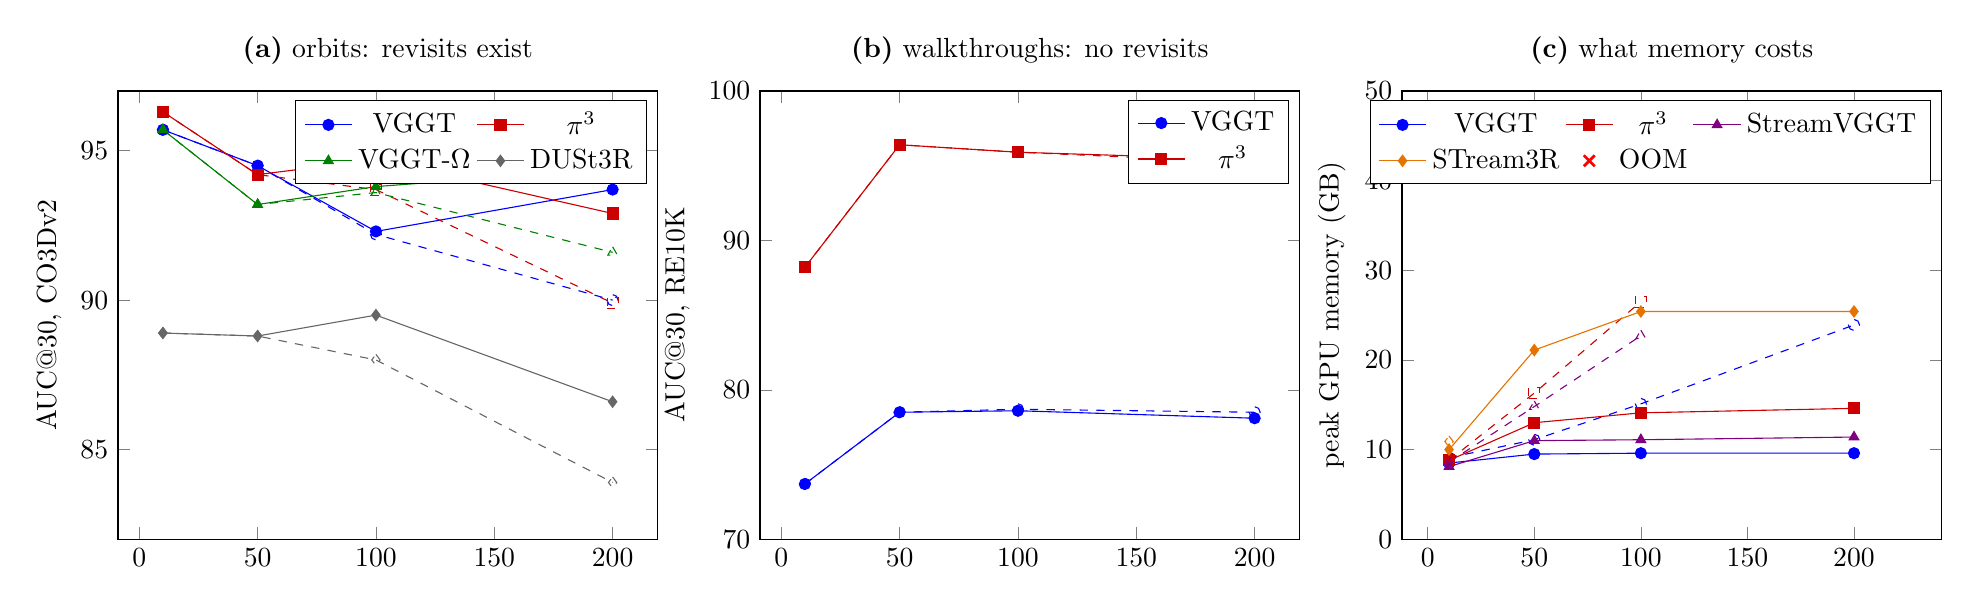
\begin{tikzpicture}
\begin{axis}[name=a, ylabel={AUC@30, CO3Dv2}, ymin=82, ymax=97, title={\textbf{(a)} orbits: revisits exist}, legend columns=2]
\addplot[blue, dashed, mark=o, forget plot] coordinates {(10,95.7)(50,94.5)(100,92.2)(200,90.0)};
\addplot[blue, mark=*] coordinates {(10,95.7)(50,94.5)(100,92.3)(200,93.7)};
\addplot[red!80!black, dashed, mark=square, forget plot] coordinates {(10,96.3)(50,94.2)(100,93.7)(200,89.9)};
\addplot[red!80!black, mark=square*] coordinates {(10,96.3)(50,94.2)(100,94.7)(200,92.9)};
\addplot[green!50!black, dashed, mark=triangle, forget plot] coordinates {(10,95.7)(50,93.2)(100,93.6)(200,91.6)};
\addplot[green!50!black, mark=triangle*] coordinates {(10,95.7)(50,93.2)(100,93.8)(200,94.4)};
\addplot[black!60, dashed, mark=diamond, forget plot] coordinates {(10,88.9)(50,88.8)(100,88.0)(200,83.9)};
\addplot[black!60, mark=diamond*] coordinates {(10,88.9)(50,88.8)(100,89.5)(200,86.6)};
\legend{VGGT, $\pi^3$, VGGT-$\Omega$, DUSt3R}
\end{axis}
\begin{axis}[name=b, at={(a.east)}, anchor=west, xshift=13mm, ylabel={AUC@30, RE10K}, ymin=70, ymax=100, title={\textbf{(b)} walkthroughs: no revisits}]
\addplot[blue, dashed, mark=o, forget plot] coordinates {(10,73.7)(50,78.5)(100,78.7)(200,78.5)};
\addplot[blue, mark=*] coordinates {(10,73.7)(50,78.5)(100,78.6)(200,78.1)};
\addplot[red!80!black, dashed, mark=square, forget plot] coordinates {(10,88.2)(50,96.4)(100,95.9)(200,95.2)};
\addplot[red!80!black, mark=square*] coordinates {(10,88.2)(50,96.4)(100,95.9)(200,95.4)};
\legend{VGGT, $\pi^3$}
\end{axis}
\begin{axis}[name=c, at={(b.east)}, anchor=west, xshift=13mm, ylabel={peak GPU memory (GB)}, ymin=0, ymax=50, title={\textbf{(c)} what memory costs}, legend columns=3]
\addplot[black!30, no marks, line width=0.6pt, forget plot] coordinates {(9,46)(220,46)} node[pos=0.5, below, font=\tiny, text=black!60] {46\,GB};
\addplot[blue, dashed, mark=o, forget plot] coordinates {(10,9.1)(50,11.1)(100,15.1)(200,23.9)};
\addplot[blue, mark=*] coordinates {(10,8.5)(50,9.5)(100,9.6)(200,9.6)};
\addplot[red!80!black, dashed, mark=square, forget plot] coordinates {(10,8.8)(50,16.3)(100,26.5)};
\addplot[red!80!black, mark=square*] coordinates {(10,8.8)(50,13.0)(100,14.1)(200,14.6)};
\addplot[violet, dashed, mark=triangle, forget plot] coordinates {(10,8.6)(50,14.8)(100,22.7)};
\addplot[violet, mark=triangle*] coordinates {(10,8.1)(50,11.0)(100,11.1)(200,11.4)};
\addplot[orange!90!black, dashed, mark=diamond, forget plot] coordinates {(10,10.9)};
\addplot[orange!90!black, mark=diamond*] coordinates {(10,10.0)(50,21.1)(100,25.4)(200,25.4)};
\addplot[only marks, mark=x, mark size=2.8pt, red, line width=1pt] coordinates {(200,46)(50,46)(100,46)};
\legend{VGGT, $\pi^3$, StreamVGGT, STream3R, OOM}
\end{axis}
\end{tikzpicture}
\vspace{-2mm}
\caption{\textbf{The thesis, measured} (cells of Tables~\ref{tab:pose} and~\ref{tab:memvsn}; dashed = raw or
native, solid = +\smr{}). (a) On CO3Dv2 orbits, raw chained windows lose accuracy with every added window;
the memory recovers most of it at $N{=}200$ and is identical to the backbone at $N{\le}50$, where no revisit
exists yet. (b) On RealEstate10K walkthroughs nothing is revisited, closures are ${\approx}0$, and the
memory correctly changes nothing --- the gain follows the mechanism. (c) Native inference pays for length in
VRAM (token cache, attention mask, alignment graph); three architectures hit the 46\,GB wall ($\times$), while
with \smr{} the cost is the window's and constant in $N$.}
\label{fig:results}
\end{figure}


Three findings, each predicted by Sec.~\ref{sec:bleed}. \textbf{The floor is
real and free.} At $N{=}10$, and at $N{=}50$ where these sequences contain no
revisit yet, all three rows are identical for every backbone---six frozen
models, zero degradation, the pass-through property measured rather than
asserted. \textbf{Beyond the window, memory pays where the mechanism
exists.} On CO3D orbits raw accuracy falls monotonically with $N$ for all six
backbones ($-4.8$ to $-7.4$ points from $N{=}10$ to $200$), and the memory
recovers most of the loss: $+3.9$ (VGGT), $+3.4$ ($\pi^3$), $+3.1$
(VGGT-$\Omega$), $+2.7$ (DUSt3R), $+1.9$ (Fast3R) at $N{=}200$, with
MASt3R---whose match-based chaining is already strong---nearly flat
($+0.2$). The causal memory alone captures $87$--$100\%$ of each gain; the
final solve adds at most $+0.4$. The one negative cell (Fast3R at
$N{=}100$, $-1.6$) is retained: its noisier per-window geometry admits
occasional wrong closures on that subset, the failure mode the consensus
gate exists to bound. \textbf{No revisits, no effect---by design.}
RealEstate10K clips are forward walkthroughs; accepted closures are
${\approx}0$ throughout, and the memory correctly changes almost nothing
($-0.4$ to $+0.3$ across all backbones and lengths). The gain tracks revisit
availability, not tuning (Fig.~\ref{fig:results}a,b).

\textbf{Streaming backbones.} Run natively on the same data, the streaming
models confirm the memory wall: StreamVGGT matches its single-window accuracy
up to $N{=}100$ and exhausts a 46\,GB GPU at $N{=}200$; STream3R exhausts it
from $N{=}50$ on CO3D. Driving the same models through \smr{}---token memory
inside each window, the bank across windows---bounds per-pass memory by the
window and restores the $N{=}200$ regime with a gain, not a compromise:
StreamVGGT $82.9\!\to\!85.9$ and STream3R $84.8\!\to\!87.6$ AUC@30 at
$N{=}200$ (Table~\ref{tab:pose}), on the exact inputs where their native
mode cannot allocate its own memory. Native accuracy also degrades with
length below the wall (StreamVGGT RE10K $81.2\!\to\!77.7$ from $N{=}10$ to
$100$): causal drift, once emitted, is unrevisable---while the composed
system's curve stays flat. Tables~\ref{tab:compute} and~\ref{tab:memvsn}
(App.~\ref{app:compute}) quantify the cost side on identical hardware: the
memory adds one $36$-frame anchored pass per accepted closure
($0.2$--$1.7$ per sequence) and a sub-second solve, and its GPU peak is the
window's, constant in $N$ (Fig.~\ref{fig:results}c). Implicit memory pays
for sequence length in VRAM; the scaffold bank pays once, in storage.

\subsection{Dense MVS and point maps: the memory inside one window}
\label{sec:mvs}
VGGT's dense benchmarks live inside a window: all 49 DTU views fit one pass,
and the ETH3D protocol uses ten frames, so pose-level memory is inert here by
construction and the DTU and ETH3D columns of Table~\ref{tab:pose} isolate
the in-window read of Sec.~\ref{sec:read}. One harness scores every row: the
official DTU evaluator with its masks and $0.2$\,mm downsampling, a Sim(3)
gauge chosen among three candidates by a symmetric fit criterion, each
backbone's native point map (its point head where it has one), and ETH3D's
official rendered depth with Umeyama alignment on per-pixel correspondences.
The protocol rows are the backbones' own output---the floor again---and the
read improves the order-dependent transformers from within: VGGT
$0.441\!\to\!0.396$\,mm on DTU (better on $23/23$ scans, landing where the
published feed-forward number stands, which neither an independent
reproduction \citep{langendoerfer2026vggt} nor ours could reach with a single
pass), VGGT-$\Omega$ $0.749\!\to\!0.655$, and, on ETH3D, VGGT
$0.490\!\to\!0.437$\,m with Accuracy nearly halved ($0.415\!\to\!0.274$). Where the orderings of a failing pass disagree, the corroborated read abstains
rather than average a failure, and abstention is what repairs the failure
scenes. The streaming
backbones, whose native passes are order-dependent too, gain on DTU
(STream3R $1.71\!\to\!1.22$, StreamVGGT $2.89\!\to\!2.25$); for
order-invariant backbones---$\pi^3$ by permutation equivariance, DUSt3R and
MASt3R by global alignment---the read is the identity and the rows are equal
by construction. Two honest cells complete the picture. The read presupposes
commensurable passes: for Fast3R and the causal models on ETH3D, different
orderings yield genuinely different reconstructions, the corroborated read
keeps too little, and the row worsens. And VGGT-$\Omega$'s ETH3D cells are
suspiciously uniform ($0.04$\,m on every scene, including the scene every
other model fails); its authors report possible benchmark contamination of
the released checkpoint, and ETH3D's training scenes are this benchmark, so
the row carries that caveat. Fusion and read policies are ablated in
App.~\ref{app:policies}, the memory's policy (sites, correction, descriptors,
scaffold size, window size) and the read's orderings in App.~\ref{app:ablations}.

\subsection{SLAM on 7-Scenes: the memory as an online system}
\label{sec:results-slam}
% NOTE: averages shared with the companion SLAM-track submission; scope
% and dual-submission framing to be confirmed before submission.
Streaming \smr{} \emph{is} an online SLAM system, and 7-Scenes
\citep{sevenscenes} lets us compare it, per trajectory ATE RMSE (m), against
dedicated pipelines (Table~\ref{tab:slam}). With its strongest frozen backbone
the memory has the best average of the table under both protocols: on seq-01
of each scene $0.030$\,m online and $0.029$ with the final solve; on all 18
trajectories of the standard test split $0.042$ and $0.038$, against
$0.042$--$0.086$ for the dedicated pipelines. The mechanism is the one this
paper is about, and the full split shows its shape honestly: chained windows
reach $0.049$; the memory recovers most where the chain drifts most (pumpkin
seq-01 $0.160\!\to\!0.077$, office seq-07 $0.144\!\to\!0.105$) and can cost
a few centimetres where the chain was already good (9 of 18 trajectories
improve online, 9 worsen slightly), the final solve recovering most of the
latter. The same machinery improves the \emph{streaming}
backbones within-session (StreamVGGT $0.133\!\to\!0.121$, STream3R
$0.089\!\to\!0.079$), and the honest column stays in view: where a whole
scene fits one native pass, the single pass is sometimes best---memory
governs what happens beyond the window, not within it. Its decisive test is
persistence: in \emph{multi-session} mapping, where the token cache dies
between sessions and the bank does not, \smr{} reduces streaming-backbone
error $4.6\times$ (StreamVGGT, $0.293\!\to\!0.064$) and $3.9\times$
(STream3R, $0.337\!\to\!0.086$)---the operation implicit memory cannot
express, measured. A companion submission develops the SLAM system itself;
here it serves as the memory's online test.

\begin{table}[t]
\centering\scriptsize
\setlength{\tabcolsep}{4.5pt}
\caption{7-Scenes SLAM, ATE RMSE (m)$\downarrow$ per scene. Published rows as
reported by their authors. Ours in two protocols: seq-01 of each scene, and
all 18 trajectories of the dataset's test split (per-scene mean of the
trajectory ATEs). Under both, \smr{} on a single frozen backbone has the best
average of the table; the largest recoveries are the trajectories whose
chains drift most (pumpkin, office seq-07). Streaming-backbone and
multi-session results are given in the text.}
% TODO(protocol): confirm which of the two protocols MASt3R-SLAM / VGGT-SLAM report; keep that block first.
\label{tab:slam}
\begin{tabular}{@{}l ccccccc c@{}}
\toprule
 & chess & fire & heads & office & pumpkin & kitchen & stairs & \textbf{avg} \\
\midrule
\multicolumn{9}{@{}l}{\emph{calibrated}} \\
NICER-SLAM~\cite{nicerslam} & 0.033 & 0.069 & 0.042 & 0.108 & 0.200 & 0.039 & 0.108 & 0.086 \\
DROID-SLAM~\cite{droidslam} & 0.036 & 0.027 & 0.025 & 0.066 & 0.127 & 0.040 & 0.026 & 0.049 \\
MASt3R-SLAM~\cite{mast3rslam} & 0.053 & 0.025 & 0.015 & 0.097 & 0.088 & 0.041 & 0.011 & 0.047 \\
\midrule
\multicolumn{9}{@{}l}{\emph{uncalibrated}} \\
VGGT-SLAM++~\cite{vggtslampp} & 0.034 & 0.023 & 0.017 & 0.104 & 0.127 & 0.085 & 0.060 & 0.064 \\
ViSTA-SLAM~\cite{vistaslam} & 0.036 & 0.033 & 0.019 & 0.103 & 0.133 & 0.058 & 0.093 & 0.067 \\
SLAM-Former~\cite{slamformer} & 0.039 & 0.033 & 0.018 & 0.070 & 0.065 & 0.035 & 0.033 & 0.042 \\
CUT3R~\cite{cut3r} & 0.046 & 0.043 & 0.055 & 0.120 & 0.096 & 0.061 & 0.086 & 0.073 \\
MASt3R-SLAM$^*$~\cite{mast3rslam} & 0.063 & 0.046 & 0.029 & 0.103 & 0.114 & 0.074 & 0.032 & 0.066 \\
VGGT-SLAM Sim(3), $w{=}32$~\cite{vggtslam} & 0.037 & 0.026 & 0.018 & 0.104 & 0.133 & 0.061 & 0.093 & 0.067 \\
VGGT-SLAM SL(4), $w{=}32$~\cite{vggtslam} & 0.036 & 0.028 & 0.018 & 0.103 & 0.133 & 0.058 & 0.093 & 0.067 \\
\midrule
\multicolumn{9}{@{}l}{\emph{VGGT-$\Omega$ (ours; uncalibrated, no backbone training) --- seq-01 of each scene}} \\
\;$w{=}32$, Sim(3) (raw) & 0.025 & 0.024 & 0.012 & 0.047 & 0.161 & 0.026 & 0.020 & 0.045 \\
\;+\smr{} & 0.022 & 0.026 & 0.012 & 0.026 & 0.077 & 0.028 & 0.022 & \textbf{0.030} \\
\;+\smr{}+PGO & 0.021 & 0.031 & 0.013 & 0.031 & 0.061 & 0.025 & 0.022 & \textbf{0.029} \\
\midrule
\multicolumn{9}{@{}l}{\emph{VGGT-$\Omega$ (ours) --- all 18 trajectories of the standard test split, per-scene mean}} \\
\;$w{=}32$, Sim(3) (raw) & 0.034 & 0.038 & 0.012 & 0.071 & 0.113 & 0.056 & 0.021 & 0.049 \\
\;+\smr{} & 0.027 & 0.026 & 0.012 & 0.073 & 0.072 & 0.061 & 0.021 & 0.042 \\
\;+\smr{}+PGO & 0.027 & 0.026 & 0.013 & 0.061 & 0.063 & 0.055 & 0.021 & \textbf{0.038} \\
\bottomrule
\end{tabular}
\end{table}

\subsection{Novel view synthesis: does corrected geometry render better?}
\label{sec:nvs}
The last evaluation asks whether the memory's geometry is worth rendering,
under the object protocol of LVSM \citep{lvsm} used by VGGT \citep{vggt}:
four input views, ten targets, PSNR/SSIM/LPIPS on GSO \citep{gso}. No renders
behind the published rows are public, so we render training objects and GSO
ourselves under one protocol (App.~\ref{app:nvs}), train one light per-pixel
Gaussian head per backbone \citep{kerbl3dgs,splatt3r} on its point maps and
images (${\approx}19$K Objaverse-LVIS objects \citep{objaverse}, $3\%$ of
Objaverse where VGGT's internal set was $20\%$), and keep the head fixed across
a backbone's rows: the read changes only the geometry the head receives.
Table~\ref{tab:nvs} gives the eight rows. The
absolute level is that of the method class: a Gaussian head over frozen
geometry lands where LGM lands, ten dB below trained transformer regressors
that hallucinate what four inputs never show. Within the rule the memory
behaves as on DTU and ETH3D. For the order-dependent
transformers the read improves the \emph{same} head with no retraining: VGGT
$20.71\!\to\!20.95$\,dB (${+}0.24$; $95\%$ bootstrap interval
$[{+}0.19,{+}0.29]$; better on $69\%$ of objects; LPIPS $-5.5\%$) and
VGGT-$\Omega$ $18.89\!\to\!19.07$ (${+}0.18$, $[{+}0.09,{+}0.26]$). For
$\pi^3$ the read is the identity to three decimals---the pass-through, measured. For the causal STream3R the mean falls by $0.18$\,dB while
the median object is unchanged and $52\%$ improve: a minority with
non-commensurable orderings pulls the mean down, as on ETH3D. The held-out Objaverse column repeats the ordering with smaller
margins (VGGT ${+}0.09$, VGGT-$\Omega$ ${+}0.05$, $\pi^3$ identity,
STream3R $-0.08$): its inputs are random training cameras rather than GSO's
four evenly spaced views, so the orderings differ less and the read has less
to reconcile. More orderings help only where they are commensurable: eight
raise VGGT by a further $0.86$\,dB and lower STream3R (App.~\ref{app:ablations}).

% Objaverse held-out cells: 174 objects, eval_gso.py --val-only (Sep 7 2026)
\newcommand{\VOr}{20.84}
\newcommand{\VOs}{0.839}
\newcommand{\VOl}{0.193}
\newcommand{\VOrR}{\textbf{20.89}}
\newcommand{\VOsR}{\textbf{0.841}}
\newcommand{\VOlR}{\textbf{0.191}}
\newcommand{\VGr}{22.79}
\newcommand{\VGs}{0.863}
\newcommand{\VGl}{0.147}
\newcommand{\VGrR}{\textbf{22.88}}
\newcommand{\VGsR}{0.863}
\newcommand{\VGlR}{0.146}
\newcommand{\PIr}{22.20}
\newcommand{\PIs}{0.857}
\newcommand{\PIl}{0.169}
\newcommand{\PIrR}{22.19}
\newcommand{\PIsR}{0.857}
\newcommand{\PIlR}{0.169}
\newcommand{\STr}{\textbf{21.15}}
\newcommand{\STs}{0.836}
\newcommand{\STl}{\textbf{0.190}}
\newcommand{\STrR}{21.07}
\newcommand{\STsR}{0.836}
\newcommand{\STlR}{0.195}
\begin{table}[t]
\centering
\scriptsize
\setlength{\tabcolsep}{4pt}
\caption{\textbf{Novel view synthesis} (four inputs, ten targets per object, $256^2$; PSNR$\uparrow$/SSIM$\uparrow$/LPIPS$\downarrow$ on
the full image over white). \emph{Objaverse-LVIS}: the 1\,\% of objects held out from the head's training (our renders,
LVSM's protocol); \emph{GSO}: all 1{,}033 objects (our renders). \emph{Top:} published rows on their authors' own
non-public renders and Objaverse-scale training sets --- anchors, not comparable. \emph{Bottom:} a frozen backbone's
point maps placed by the known input cameras and one light Gaussian head per backbone (${\approx}19$K Objaverse-LVIS
objects, ${\approx}3\%$). raw = single pass; +\smr{} = the in-window read through the \emph{same} head, so a row
difference is a geometry difference. One window has no junction graph, so no +\smr{}+PGO variant exists. Bold: better of each pair (differences within $0.01$\,dB / $0.001$ are ties).}
\label{tab:nvs}
\begin{tabular}{@{}l c c ccc ccc@{}}
\toprule
& & & \multicolumn{3}{c}{Objaverse-LVIS (held out)} & \multicolumn{3}{c}{GSO} \\
\cmidrule(lr){4-6}\cmidrule(lr){7-9}
Method & known input cams & training set & PSNR & SSIM & LPIPS & PSNR & SSIM & LPIPS \\
\midrule
\multicolumn{9}{@{}l}{\emph{published (authors' renders; not comparable to the rows below)}} \\
LGM \citep{lgm} & \checkmark & Objaverse renders & -- & -- & -- & 21.44 & 0.832 & 0.122 \\
GS-LRM \citep{gslrm} & \checkmark & Objaverse renders (730K) & -- & -- & -- & 29.59 & 0.944 & 0.051 \\
LVSM \citep{lvsm} & \checkmark & Objaverse renders (730K) & -- & -- & -- & 31.71 & 0.957 & 0.027 \\
VGGT-NVS \citep{vggt} & $\times$ & internal, ${\approx}20\%$ Objaverse & -- & -- & -- & 30.41 & 0.949 & 0.033 \\
\midrule
\multicolumn{9}{@{}l}{\emph{ours (our renders; ${\approx}19$K Objaverse-LVIS objects, ${\approx}3\%$; frozen backbone $+$ Gaussian head)}} \\
VGGT-$\Omega$ (raw) & \checkmark & Objaverse-LVIS (19K) & \VOr{} & \VOs{} & \VOl{} & 18.89 & 0.796 & 0.204 \\
\;+\smr{} & \checkmark & & \VOrR{} & \VOsR{} & \VOlR{} & \textbf{19.07} & \textbf{0.799} & \textbf{0.200} \\
VGGT (raw) & \checkmark & Objaverse-LVIS (19K) & \VGr{} & \VGs{} & \VGl{} & 20.71 & 0.821 & 0.152 \\
\;+\smr{} & \checkmark & & \VGrR{} & \VGsR{} & \VGlR{} & \textbf{20.95} & \textbf{0.823} & \textbf{0.143} \\
$\pi^3$ (raw) & \checkmark & Objaverse-LVIS (19K) & \PIr{} & \PIs{} & \PIl{} & 21.91 & 0.844 & 0.132 \\
\;+\smr{} & \checkmark & & \PIrR{} & \PIsR{} & \PIlR{} & 21.91 & 0.844 & 0.132 \\
STream3R (raw) & \checkmark & Objaverse-LVIS (19K) & \STr{} & \STs{} & \STl{} & \textbf{18.79} & \textbf{0.784} & \textbf{0.209} \\
\;+\smr{} & \checkmark & & \STrR{} & \STsR{} & \STlR{} & 18.60 & 0.781 & 0.222 \\
\bottomrule
\end{tabular}
\vspace{-3mm}
\end{table}


% Figure 3 placeholder: qualitative NVS (inputs | raw render | +SMR render | GT), 2 objects.
% \begin{figure}[t]\centering\includegraphics[width=\textwidth]{fig_nvs_qual.pdf}
% \caption{...}\label{fig:nvs}\end{figure}

\section{Limitations}
\label{sec:limitations}
The memory helps only where its mechanism exists: without revisits it is,
correctly, inert (RealEstate10K), and its gains are bounded by what the
backbone can re-measure. The in-window read presupposes commensurable passes;
for models whose reconstruction depends on the reference frame or the causal
order (Fast3R, StreamVGGT, STream3R) the orderings disagree and the read
keeps too little or averages incompatible geometry---a failure we report
rather than remove. Two-site consensus is defeated by look-alike structures that also agree
geometrically; one wrong closure survived the gate on a Fast3R subset. The bank's storage grows with the scene
(in cards, not VRAM); we have not studied forgetting, and hyperparameters are
conventional defaults without sweeps. Our NVS rows use our own renders and sit
at the level of Gaussian heads over frozen geometry, ten dB below trained
transformer regressors.

\vspace{-1mm}
\section{Conclusion}
\vspace{-1mm}
Geometry foundation models did not need a better eye; they needed a memory
that can correct. We built one from a grid-cell scaffold whose dynamics
settle what is internally inconsistent and are blind to what is merely
elsewhere, and completed it with the only instrument these models leave
us---themselves. The result is gradient-free, backbone-agnostic, bit-identical
to the model within its window, and beyond it recovers most of what seams
destroy, improves a single pass by reading repeated writes, gives streaming
models the long regime their caches cannot afford, and runs as a SLAM system with the best average error on 7-Scenes. What remains is the memory's own biology:
consolidation, forgetting, and whether a scaffold trained nowhere can, given
the right measurements, remember anywhere.

\vspace{-3mm}
\subsubsection*{Reproducibility statement}
\vspace{-1mm}
Hyperparameters (one setting for all tasks and backbones) are listed with
their motivation in App.~\ref{app:repro}; protocols per benchmark in
Secs.~\ref{sec:results-pose}--\ref{sec:nvs} and Apps.~\ref{app:policies},~\ref{app:nvs}.
Backbones use public weights unmodified, randomness is seeded, and every run
writes a JSON report (metrics, accepted and rejected closures, solver
diagnostics); code and scripts will be released.

\vspace{-3mm}
\subsubsection*{Ethics statement}
\vspace{-1mm}
Only public benchmark imagery is used (CO3Dv2, RealEstate10K, DTU, ETH3D,
7-Scenes, Objaverse, GSO), under its licenses; no data involving people is
collected. A persistent memory of places is dual-use (mapping, but also
surveillance); it stores geometry and appearance, not identities.

\bibliography{references}
\bibliographystyle{iclr2027_conference}

\appendix
\section{Notation and $\simthree$ operations}
\label{app:sim3}
A similarity $S=(s,R,t)\in\simthree$ acts on points as $S\cdot x = sRx+t$
and on a camera-to-world pose $g=(R_g,t_g)$ as
$S\cdot g = (R R_g,\; sRt_g + t)$: rotations compose, positions are scaled
and moved, and the local frame's scale is absorbed into the map. We write
$\mathrm{Log}:\simthree\to\mathbb{R}^7$ for the logarithm splitting into
rotation angle-axis $\omega\in\mathbb{R}^3$, translation $\nu\in\mathbb{R}^3$,
and log-scale $\sigma\in\mathbb{R}$.

\paragraph{Closed-form alignment.}
Given corresponding pose sets $\{(g_j^{A}, g_j^{B})\}_{j=1}^{n}$ (the same
physical frames expressed in two gauges), the alignment
$\hat S=\argmin_S \sum_j \|S\cdot c_j^{A} - c_j^{B}\|^2$ over camera
centres $c_j$ has the closed-form solution of \citet{umeyama} (rotation by
SVD of the centred cross-covariance with a determinant sign correction
\citep{horn}, scale by variance ratio, translation by centroids).

\paragraph{Robust IRLS wrapper.}
Pose sets contain occasional gross errors, so we wrap the closed form in
iteratively reweighted least squares: initialize with all pairs; at each of
$T{=}5$ rounds compute residuals $r_j = \|\hat S\cdot c^A_j - c^B_j\|$,
set Huber weights $w_j=\min(1, \kappa\,\tilde r/r_j)$ with $\tilde r$ the
median residual and $\kappa{=}2.5$, and re-solve on weighted centroids.
Rotational agreement is checked on the fitted $R$: pairs whose relative
rotation residual exceeds $\theta_{\max}$ are dropped. The fit is declared
valid only if (i) at least $n_{\min}{=}4$ inliers remain and (ii) the
\emph{scale gate} passes: the ratio between the fitted scale and the
median pairwise-distance ratio lies in $[1/\gamma_s,\gamma_s]$
($\gamma_s{=}1.5$). Fits failing the gate are discarded rather than
down-weighted; a wrong scale poisons everything downstream.

\section{Windowed inference, junctions, and the invariant}
\label{app:invariant}
\paragraph{Keyframing and windows.}
Keyframes are taken at a fixed temporal stride; windows are consecutive
runs of $W$ keyframes overlapping by $O$ (defaults $W{=}32$, $O{=}16$;
per-dataset strides in App.~\ref{app:repro}). Each keyframe $j$ is
\emph{owned} by the first window covering it, $k(j)$; overlap frames thus
belong to two windows but are owned by one, and every stored pose
$g_j^{(k(j))}$ is expressed in its owner's gauge.

\paragraph{Junction edges.}
For consecutive windows the shared frames give correspondences for
Eq.~\ref{eq:junction}; the resulting $\hat S_{k,k+1}$ becomes a
\emph{sequential edge} $Z=\hat S_{k,k+1}$ between nodes $k,k{+}1$. When the
overlap exceeds half the window, overlap frames span two previous windows;
edges sourced from overlap frames are sequential regardless of owner
distance (only anchor-sourced constraints are loop edges).

\paragraph{Why the pass-through property holds.}
(a) $N\le W$: one window, one node, no junction edges; the revisit gap
$\Delta$ (measured in keyframes) excludes all frames of the same window
from proposal, so the memory proposes nothing; the pose graph over a
single node has the identity as optimum in any gauge convention; frames
inherit $\hat g_j = T_1 g_j^{(1)}$ with $T_1$ the gauge anchor---the
backbone's output up to the global frame, i.e., exactly the backbone's
output under the benchmark's gauge-free metrics. (b) General case: \smr{}
computes $\hat g_j = T_{k(j)} g_j^{(k(j))}$; for $j,j'$ with
$k(j){=}k(j'){=}k$, the relative pose
$\hat g_{j'}^{-1}\hat g_j = (g^{(k)}_{j'})^{-1} (T_k^{-1}T_k)\, g^{(k)}_j$
equals the backbone's within-window relative pose; rotation and translation
direction are invariant to the window's similarity placement.

\section{The scaffold memory: instantiation, loop, and relation to Vector-HaSH}
\label{app:vhash}

\subsection{Fields, modules, and sizes}
Every ring and torus is an Amari-type neural field integrated forward in
time (bump width ${\approx}8$ units on a $48$ grid). The configuration
used in all experiments (\texttt{compact}) has three spatial modules,
each a $48{\times}48$ torus (horizontal phase) plus a $48$-unit height
ring, and three head-direction rings of $256$ units (ZYX Euler) driven
through the rotation gate $R(\hat\psi,\hat\theta,\hat\phi)$, the unique
gating making phase increments exact differentials (measured $9.3\times$
gap over alternatives). The joint code is
$\mathbf g\in\mathbb R^{N_g}$ with
$N_g = 3\times(48^2{+}48) + 3\times256 = 7{,}824$. Periods
$\{2.4,3.2,4.0\}$ (normalized scene units, median depth ${:=}1$) form the
smallest coprime ladder $3{:}4{:}5$, giving a Chinese-remainder
unambiguous range of $2.4\cdot\mathrm{lcm}(3,4,5)=144$ units---beyond
every benchmark scene. Range multiplies per added module (the shipped
\texttt{default} adds $\lambda{=}5.6$, $N_g{=}10{,}176$; a six-module
plan-scale point, $N_g{=}14{,}880$, exists as design headroom and is not
used in any reported experiment): scaling is additive hardware, not
retuning.

\subsection{The consistency loop and what it corrects}
$\mathbf g$ is projected to a sparse hippocampal layer through a
\emph{fixed random} matrix and returned through an associative map,
\begin{equation}
\mathbf h=\sigma(W_{gh}\,\mathbf g),\qquad
\hat{\mathbf g}=\psi(W_{hg}\,\mathbf h),
\end{equation}
with $\sigma$ a top-$k$ threshold ($N_h{=}1024$, $k{=}64$ active; a scaled variant, $8192/410$, is available and unchanged in behavior) and $\psi$ per-field
normalization back to a valid population code. For the sparse binary
codes of Vector-HaSH a Hebbian sum approximates the return map; for our
\emph{continuous} field templates the Hebbian sum is at chance, and the
ridge form $W_{hg}=G(H^{\!\top}H+\lambda I)^{-1}H^{\!\top}$ is the
faithful pseudoinverse implementation (verified empirically). Formation
visits states \emph{covering every per-module phase} at spacing
$\le\lambda_{\min}/6$ (six samples per period per axis---the measured
covering condition) over a formation extent of $1.2$ normalized units;
thereafter all $\prod_m\lambda_m$ joint states are attractors provided
$N_h\ge N_h^{\!*}$, with $N_h^{\!*}$ linear in $M$ and nearly independent
of period; we set $N_h\ge4\times$ the measured $N_h^{\!*}$.

The loop's power is \emph{selective}, and the selectivity organizes the
whole system. Perturbations of the joint fiber split into a
\emph{coherent} subspace---module shifts explicable by one spatial
displacement, which describe another perfectly legitimate location and are
internally invisible---and its \emph{incoherent} complement, module
combinations that agree with no location. Settling through the loop
corrects exactly the incoherent part; the coherent part can only be pinned
by external observation. \smr{} supplies that pin: every input view is
\emph{anchored} at its backbone pose (a localized clamp input---anchoring,
not state overwrite), and verified loop closures re-pin the past. The
attractor loop and the geometric machinery of App.~\ref{app:closure} are
thus not alternatives but a division of labor: dynamics absorb incoherent
drift continuously; placement and closure correct the coherent drift that
dynamics cannot see.

\paragraph{Argument for Proposition~\ref{prop:coherent}.}
Let $\Phi(\gvec)=\psi(W_{hg}\,\sigma_k(W_{gh}\,\gvec))$ be the loop. Formation
fits $W_{hg}$ by ridge regression so that $\Phi(\gvec_p)=\gvec_p$ for the
template code $\gvec_p$ of every joint phase $p$ on the formation lattice; the
per-field normalization $\psi$ maps any output onto the manifold $\mathcal M$
of valid population codes (one bump per field), and the lattice covers each
module's phase at spacing $\le\lambda_{\min}/6$, the measured covering
condition under which the interpolation error of $\Phi$ between lattice
templates stays below the bump width, so every point of $\mathcal M$ is (to
numerical precision) a fixed point. A perturbation $\delta$ of a stored code
$\gvec_p$ decomposes as $\delta=\delta_{\parallel}+\delta_{\perp}$ with
$\gvec_p+\delta_{\parallel}\in\mathcal M$ (a coherent shift: one displacement
applied to every module, i.e., the code of another location) and
$\delta_{\perp}$ transverse to $\mathcal M$ (module states that agree with no
single location). Since $\gvec_p+\delta_{\parallel}$ is itself a fixed point,
$\Phi$ leaves it unchanged; since $\mathcal M$ is the attracting set of $\Phi$
(empirically, with a contraction factor below one for the transverse component
at every tested $N_h\ge N_h^{*}$), iterating $\Phi$ removes $\delta_{\perp}$.
The loop is therefore exactly as strong as it is blind: it cannot distinguish
$\gvec_p+\delta_{\parallel}$ from a legitimate memory of another place, and
only a clamp---an input pinning a field to an externally measured phase---can
correct it. This is the operational content of Vector-HaSH's
coherent/incoherent split, restated for continuous fields and used as a design
rule rather than a theorem about capacity.

\subsection{Indexing: cards, not photocopies}
Following the library principle, the hippocampal layer does not store
content. Each bound state associates the scaffold code with a
\emph{card}: a $448$-dimensional cue descriptor plus an index code
addressing the bank, where the actual content lives: owner window, owner-gauge pose, surfels, and per-primitive appearance features consumed by the supervised recall-side renderer. Scenes coexist through per-module remap offsets, so one scaffold serves many scenes.
This indexing substitution is the one structural
change relative to Vector-HaSH, and it is what lets the same scaffold
serve arbitrarily heavy content (full surfel sets) at fixed loop cost.

\subsection{Cues, novelty, and retrieval}
\label{app:cue}
\paragraph{The scaffold cue.}
The cue keying each bound state is a $448$-dimensional engineered
descriptor: a $192$-d color thumbnail, $144$-d grey structure bands, and
$48$-d intensity histograms, $\ell_2$-normalized per block so that
natural magnitudes act as implicit weights. Two seemingly reasonable
enrichments were tested and rejected by measurement: appending a depth
channel and learning a re-weighting both \emph{reduced} retrieval on the
held-out probe (from $97.5\%$ correct to $64.5\%$ with the depth
channel), because both couple the cue to quantities that vary with the
backbone and the gauge. The long-range revisit proposals of the
stitcher use a frozen self-supervised global descriptor
\citep{dinov2} over the same bank. We do not key memory on the
backbone's own features for a structural reason: the cue must be
identical across backbones for one bank to serve six models, and it must
remain valid if the backbone is swapped; pooled backbone features remain
a candidate replacement and will be adopted only if they match the
engineered cue on the retrieval probe.

\paragraph{Novelty gate.}
A view is bound only if its cue similarity to every stored card is below
$\tau=\max(0.2,\,3\times\mathrm{floor})$, where the floor is the
similarity of unrelated views, probed at bind time from lattice
midpoints of the current scene. The floor is probed rather than fixed
because a constant threshold, tuned on one scene family, produced a
false ``familiar'' verdict in deployment on another.

\paragraph{Two-stage retrieval.}
Recall proposes the top-$5$ scaffold matches by cue similarity and
verifies each geometrically (App.~\ref{app:closure}) before any is
used. In the controlled cue-corruption test (cosine ${\approx}0.71$ to
the true cue), single-shot recall returned the correct state in $22$ of
$39$ probes; propose-and-verify returned $39$ of $39$. Verification is
not a safeguard bolted on---it is the recall mechanism appropriate to a
continuous state space, where the nearest attractor is not guaranteed to
be the right one.

\section{Closure: proposal, anchored re-measurement, consensus}
\label{app:closure}
\paragraph{Sites.}
A proposal $(q, j_{\text{old}})$ defines a site
$\{\,j_{\text{old}},\, j_{\text{old}}{+}\delta\,\}$ (partner offset
$\delta{=}3$ keyframes; the partner disambiguates orientation and provides
baseline). Up to $n_s{=}2$ sites from distinct old frames are attached per
window per proposal round.

\paragraph{Anchored pass and the closure estimate.}
Let $\cA = \cW_k \cup \text{sites}$. One backbone pass on $\cA$ yields
poses $\{h_i\}_{i\in\cA}$ in the anchored gauge. Two robust fits
(App.~\ref{app:sim3}) give
$S_{\cA\to k}$ (anchored $\to$ window-$k$ gauge, over $\cW_k$'s frames) and
$S_{\cA\to o}$ (anchored $\to$ owner gauge of the site, over site frames,
matched to their stored $g^{(k(j_{\text{old}}))}$). The candidate closure
between nodes is
\begin{equation}
\hat Z \;=\; S_{\cA\to o}\; S_{\cA\to k}^{-1}
\;\in\;\simthree ,
\end{equation}
mapping window-$k$ coordinates into the old owner's coordinates. Site fits
use $n{=}2$ frames plus the window-side redundancy; the scale gate of
App.~\ref{app:sim3} applies to both fits.

\paragraph{Two-site consensus.}
Sites $a,b$ yield $\hat Z_a,\hat Z_b$ and implied placements
$T_k^{(a)},T_k^{(b)}$ of the new window. Acceptance requires
\begin{equation}
\angle\big(R(T_k^{(a)}),R(T_k^{(b)})\big) \le \theta_{\text{agree}},
\qquad
\big\|c(T_k^{(a)})-c(T_k^{(b)})\big\| \le \lambda_{\text{agree}}\cdot E,
\end{equation}
with $E$ the current map extent (scene-relative tolerance). Independent
wrong matches rarely agree; look-alike structures that defeat this gate
(repetitive facades) are the recorded failure mode, and any residual wrong
closure is exposed to the batch solver's rejection round. Accepted closures
add a loop edge $Z=\hat Z$ (consensus-averaged over agreeing sites) with a
scale weight reflecting the site fit's confidence; rejected proposals are
logged with their disagreement.

\section{Pose-graph objective and solvers}
\label{app:pgo}
Variables are node placements $T_1,\dots,T_K\in\simthree$ ($T_1$ fixed as
gauge). Each edge $e=(c,k,Z_e,w_e)$ contributes the residual
\begin{equation}
r_e(T) \;=\; \mathrm{Log}\!\big(Z_e^{-1}\, T_c^{-1} T_k\big)
\;=\;(\omega_e,\nu_e,\sigma_e)\in\mathbb{R}^{7},
\end{equation}
weighted componentwise: rotation and translation by edge type, log-scale by
$w_e$ (sequential edges measure scale reliably from many shared frames,
$w_e{=}1$; loop-edge scale from two-frame sites is down-weighted). The
batch objective is
\begin{equation}
\min_{T_2..T_K}\; \sum_e \rho_{\text{H}}\!\big(\|r_e(T)\|_{\Lambda_e}\big),
\end{equation}
with Huber $\rho_{\text{H}}$ \citep{huber}, solved by Levenberg--Marquardt
on the $7(K{-}1)$-dimensional parameterization from the chained
initialization. A \emph{rejection round} follows: edges whose robust
residual exceeds a multiple of the median are removed and the problem is
re-solved once \citep{grisetti}; the count of dropped edges is reported.

\paragraph{Streaming relaxation.}
Online, an accepted closure at window $k$ against owner $o$ implies a
correction $C = T_o Z\, \big(T_k^{\text{pred}}\big)^{-1}$. \smr{}
distributes $\mathrm{Log}\,C$ over the intervening nodes
$o{+}1,\dots,k$ with linearly increasing fractions (rotation, translation,
and log-scale interpolated in the tangent space), leaving nodes outside the
span untouched: cost $O(k-o)$ per closure, causal, and equivalent to one
Gauss--Seidel sweep of the batch problem restricted to the span. All
reported ``streaming'' results use only this rule; ``batch'' adds the full
solve above at sequence end.

\section{Surfels, rendering, and fusion}
\label{app:surfel}
\paragraph{Construction.}
For an owned frame $j$, pixels on a stride grid with valid depth are
unprojected: $x = g_j^{(k(j))}\cdot \pi^{-1}(u; D_j(u), K_j)$, carrying the
pixel color and an isotropic footprint from the local depth gradient. The
global position of every surfel is $T_{k(j)}\cdot x$---stored once in the
owner gauge, re-embedded for free whenever the solver updates $T$.

\paragraph{Rendering (used by relocalization visualization and NVS
conditioning).}
Surfels are projected into a target camera with a z-buffer and a small
square splat (2--3\,px) for hole suppression---classical point splatting
\citep{surfels}, not 3D Gaussian splatting; no covariances or opacities are
stored or optimized. The renderer is deterministic and differentiable-free.

\paragraph{Cross-window fusion for depth/point benchmarks.}
\label{app:fusion}
For multi-view depth and point-map evaluation, $k$ overlapping windows over
the view set are bound as above; alignment across windows uses pose-head
junctions only. For each target pixel, candidate 3D points from all windows
containing the view are collected; a point is kept if at least $m{=}2$
windows agree within $\tau_{\text{fuse}}$ (relative to depth), and the
fused estimate is the coordinate-wise median of the agreeing set.
Consistency filtering targets accuracy; multi-window coverage protects
completeness. Depth is never used to estimate any transform---the
alignment-versus-estimand separation is a design rule motivated by six
recorded negative results in development, in which every densification of
the \emph{alignment} channel (3D--3D edges, dense placement, long-span pose
fits) degraded accuracy due to correlated per-pass error.

\section{Compute and memory measurements}
\label{app:compute}
Tables~\ref{tab:compute} and~\ref{tab:memvsn} give the resource side of
Sec.~\ref{sec:results-pose} on identical hardware (one RTX 6000 Ada, 46\,GB,
batch 1, public weights). The pattern is the thesis in resource units: native
inference pays for input length in VRAM---token cache (StreamVGGT), attention
mask (STream3R), pairwise-alignment graph (DUSt3R/MASt3R)---and three
architectures hit the wall inside the studied range, while the composed
system's peak is the window's and constant in $N$. The memory's own cost is
one $36$-frame anchored pass per accepted closure ($0.2$--$1.7$ closures per
sequence, measured per backbone) and a sub-second robust solve.

\begin{table}[h]
\centering\scriptsize
\setlength{\tabcolsep}{3.5pt}
\caption{Compute at $N{=}100$ input frames on one RTX 6000 Ada (46\,GB),
batch 1, public weights. \emph{native}: one $N$-frame inference, all
columns measured by the probe (host-RAM per-pass delta ${\approx}0$;
peak is reached at weight load). \emph{raw}: Sim(3)-chained windows,
wall time measured cold during the Table~\ref{tab:pose} runs.
\emph{+\smr{}}: raw $+$ its measured memory overhead---per accepted
closure ($0.2$--$1.7$/sequence, measured per backbone) one 36-frame
anchored pass at the probe-measured unit time---and \emph{+PGO} adds the
measured end-to-end solver-stage delta. GPU peaks are per-variant
measurements from the same runs. $^{c}$CPU seconds and GFLOPs of
windowed rows compose measured 32/36-frame unit passes
($n_{\mathrm{win}}{=}6$). $^{e}$end-to-end stage time; the Sim(3) solve
itself is ${<}1$\,s (App.~\ref{app:pgo})---the remainder is harness
re-evaluation for the pairwise backbones. $^{s}$,$^{d}$: see
Table~\ref{tab:memvsn}.}
\label{tab:compute}
\begin{tabular}{@{}l rrrrr@{}}
\toprule
Model & CPU (s) & GPU (GB) & GFLOPs & Time (s) & s/frame \\
\midrule
DUSt3R (native) & \multicolumn{5}{c}{n/f: pairwise global alignment (host-RAM/time wall)} \\
\;raw, windowed & 2447$^{c}$ & 25.8 & 10{,}577{,}648$^{c}$ & 732.8 & 7.33 \\
\;+\smr{} & 3166$^{c}$ & 28.8$^{d}$ & 13{,}712{,}530$^{c}$ & 1020.8 & 10.21 \\
\;+\smr{}+PGO & 3166$^{c}$ & 28.8 & 13{,}712{,}530$^{c}$ & 1559.9$^{e}$ & 15.60 \\
\midrule
Fast3R (native) & 50.1 & 13.9 & 662{,}924 & 8.0 & 0.08 \\
\;raw, windowed & 106$^{c}$ & 9.1 & 577{,}570$^{c}$ & 22.0 & 0.22 \\
\;+\smr{} & 132$^{c}$ & 9.2 & 705{,}528$^{c}$ & 24.9 & 0.25 \\
\;+\smr{}+PGO & 132$^{c}$ & 9.2 & 705{,}528$^{c}$ & 29.8 & 0.30 \\
\midrule
MASt3R (native) & \multicolumn{5}{c}{n/f: pairwise global alignment (host-RAM/time wall)} \\
\;raw, windowed & 2181$^{c}$ & 7.1 & 9{,}322{,}638$^{c}$ & 1067.4 & 10.67 \\
\;+\smr{} & 2274$^{c}$ & 7.6$^{d}$ & 11{,}890{,}239$^{c}$ & 1109.1 & 11.09 \\
\;+\smr{}+PGO & 2274$^{c}$ & 7.6 & 11{,}890{,}239$^{c}$ & 1894.7$^{e}$ & 18.95 \\
\midrule
VGGT (native) & 32.9 & 15.1 & 2{,}201{,}982 & 19.9 & 0.20 \\
\;raw, windowed & 50$^{c}$ & 9.5 & 1{,}804{,}796$^{c}$ & 25.1 & 0.25 \\
\;+\smr{} & 66$^{c}$ & 9.6 & 2{,}436{,}362$^{c}$ & 32.3 & 0.32 \\
\;+\smr{}+PGO & 66$^{c}$ & 9.6 & 2{,}436{,}362$^{c}$ & 42.5 & 0.43 \\
\midrule
VGGT-$\Omega$ (native) & 24.0 & 11.9 & 1{,}079{,}048 & 11.3 & 0.11 \\
\;raw, windowed & 41$^{c}$ & 6.8 & 944{,}944$^{c}$ & 19.1 & 0.19 \\
\;+\smr{} & 52$^{c}$ & 6.9 & 1{,}257{,}536$^{c}$ & 22.9 & 0.23 \\
\;+\smr{}+PGO & 52$^{c}$ & 6.9 & 1{,}257{,}536$^{c}$ & 29.3 & 0.29 \\
\midrule
$\pi^3$ (native) & 28.4 & 26.5 & 1{,}519{,}345 & 16.7 & 0.17 \\
\;raw, windowed & 46$^{c}$ & 13.0 & 1{,}349{,}872$^{c}$ & 25.3 & 0.25 \\
\;+\smr{} & 58$^{c}$ & 14.1 & 1{,}824{,}876$^{c}$ & 31.0 & 0.31 \\
\;+\smr{}+PGO & 58$^{c}$ & 14.1 & 1{,}824{,}876$^{c}$ & 42.0 & 0.42 \\
\midrule
StreamVGGT (native) & 49.8 & 22.7 & 1{,}283{,}334 & 37.0 & 0.37 \\
\;raw, windowed & 56$^{c}$ & 11.0 & 1{,}252{,}493$^{c}$ & 24.9 & 0.25 \\
\;+\smr{} & 72$^{c}$ & 11.1 & 1{,}587{,}905$^{c}$ & 33.9 & 0.34 \\
\;+\smr{}+PGO & 72$^{c}$ & 11.1 & 1{,}587{,}905$^{c}$ & 46.3 & 0.46 \\
\midrule
STream3R (native) & \multicolumn{5}{c}{OOM: mask allocation requests 70.3\,GiB} \\
\;raw, windowed & 67$^{c}$ & 21.1 & 1{,}804{,}796$^{c}$ & 29.9 & 0.30 \\
\;+\smr{} & 88$^{c}$ & 25.4$^{s}$ & 2{,}357{,}416$^{c}$ & 42.9 & 0.43 \\
\;+\smr{}+PGO & 88$^{c}$ & 25.4 & 2{,}357{,}416$^{c}$ & 59.0 & 0.59 \\
\bottomrule
\end{tabular}
\end{table}

\begin{table}[h]
\centering\scriptsize
\setlength{\tabcolsep}{4pt}
\caption{GPU peak memory (GB) versus input length $N$: one native
$N$-frame inference (probe, measured per $N$) against the composed
system's measured peak over its actual 32/36-frame passes at that $N$
(from the Table~\ref{tab:pose} runs). Native cost grows for every
architecture and walls for three of them---token cache (StreamVGGT,
$N{=}200$), attention mask (STream3R, $N{\ge}50$), pairwise-alignment
graph (DUSt3R/MASt3R, n/f beyond $N{=}50$)---while +\smr{} is constant
in $N$ at the window/anchored-pass cost. $^{s}$one-time step from the
${\le}W$ single pass to the 32/36-frame pass; constant thereafter.
$^{d}$DUSt3R/MASt3R windowed peaks drift ${\sim}0.1$--$0.7$\,GB per
additional window (allocator retention in their alignment code), not
context growth.}
\label{tab:memvsn}
\begin{tabular}{@{}l rr rr rr rr@{}}
\toprule
 & \multicolumn{2}{c}{$N{=}10$} & \multicolumn{2}{c}{$N{=}50$}
 & \multicolumn{2}{c}{$N{=}100$} & \multicolumn{2}{c}{$N{=}200$} \\
Model & nat. & +\smr{} & nat. & +\smr{} & nat. & +\smr{} & nat. & +\smr{} \\
\midrule
DUSt3R & 4.9 & 4.4 & OOM & 25.8$^{d}$ & n/f & 28.8$^{d}$ & n/f & 32.1$^{d}$ \\
Fast3R & 6.3 & 5.7 & 11.4 & 9.1 & 13.8 & 9.2 & 18.7 & 9.2 \\
MASt3R & 3.2 & 3.2 & 20.7 & 6.7 & n/f & 7.6$^{d}$ & n/f & 8.8$^{d}$ \\
VGGT & 9.1 & 8.5 & 11.1 & 9.5 & 15.1 & 9.6 & 23.9 & 9.6 \\
VGGT-$\Omega$ & 5.7 & 5.7 & 8.1 & 6.8 & 11.9 & 6.9 & 19.5 & 7.0 \\
$\pi^3$ & 8.8 & 8.8 & 16.3 & 13.0 & 26.5 & 14.1 & OOM & 14.6 \\
StreamVGGT & 8.6 & 8.1 & 14.8 & 11.0 & 22.7 & 11.1 & OOM & 11.4 \\
STream3R & 10.9 & 10.0 & OOM & 21.1$^{s}$ & OOM & 25.4$^{s}$ & OOM & 25.4$^{s}$ \\
\bottomrule
\end{tabular}
\end{table}

\section{Novel view synthesis: protocol, renderer, head}
\label{app:nvs}
\paragraph{Protocol.} We follow the object protocol of LVSM \citep{lvsm} and
VGGT \citep{vggt}: four input views and ten target views per object, scored by
PSNR, SSIM and LPIPS \citep{lpips} on the full $256^2$ image composited on
white. GSO \citep{gso} is the test set. The published rows of
Table~\ref{tab:nvs} were computed on their authors' renders (Objaverse and GSO
renders for GS-LRM/LVSM; an internal set for VGGT-NVS), none of which is
public, so our rows are computed on our own renders under one stated protocol
and compared among themselves.

\paragraph{Renders.} Objects are normalized to a bounding sphere of radius
$0.5$ at the origin; cameras lie on a sphere of radius $2.0$ with a vertical
field of view of $40^\circ$ (the object always fits: the ball subtends
$29^\circ$); images are $256^2$, OpenCV camera convention in a $y$-up world.
Training objects: ${\approx}20$K Objaverse-LVIS objects \citep{objaverse},
sampled round-robin over the 1{,}156 LVIS categories with a fixed seed
(${\approx}3\%$ of Objaverse; VGGT used an internal set of ${\approx}20\%$),
$16$ views each at azimuth $\sim U(0,360^\circ)$ and elevation
$\sim U(-20^\circ,60^\circ)$. GSO: four inputs at elevation $20^\circ$ and
azimuths $0/90/180/270^\circ$ plus ten targets drawn as training views with a
per-object seed. Renderer: Blender Cycles (GPU, 32 adaptive samples,
denoised), a white world plus one sun fixed per object, standard view
transform, RGBA output whose alpha is the object mask; the same renderer
produces training and test images.

\paragraph{Geometry.} The frozen backbone runs on the four input images; each
view's predicted depth (or point head, expressed in that view's camera) is
unprojected through the \emph{known} input camera, with the metric scale given
by the Sim(3) fitting the four predicted cameras to the four given ones (the
``known input cameras'' setting of GS-LRM/LVSM). Maps are resampled from the
backbone grid to the render grid; the square image is never cropped. The
+\smr{} row applies the in-window read of Sec.~\ref{sec:read}: four orderings
of the same views, symmetric re-measure of each pass's scale about the given
cameras, per-pixel consensus by the median of the witnesses---the same
functions as the DTU/ETH3D rows.

\paragraph{Head and training.} A per-pixel Gaussian head \citep{kerbl3dgs} in
the spirit of Splatt3R \citep{splatt3r}: a small U-Net (${\approx}1.2$M
parameters) over eight input channels (rgb, world $xyz$, depth, confidence)
predicts, for every valid pixel (object mask and finite geometry), a position
offset bounded to $0.02$ ($4\%$ of the object radius, so the backbone's
geometry stays in charge), log-scales about one pixel footprint, a rotation,
an opacity, and a colour residual on the input colour; the output layer is
zero-initialized so training starts from ``splat the backbone's coloured
points''. Gaussians are rasterized with gsplat into the target cameras on a
white background. One head per backbone, trained on raw geometry for $30$K
steps (one object per step, four inputs and four random targets, AdamW
$2\times10^{-4}$ with warm-up and cosine decay, MSE $+\,0.1\,$LPIPS), then
evaluated with raw and with read geometry unchanged. The head is deliberately
light: the question is whether corrected geometry renders better through a
fixed decoder, not how far a decoder can be pushed.

\section{Related work}
\label{app:related}
\paragraph{Feed-forward geometry.} DUSt3R and MASt3R \citep{dust3r,mast3r}
regress pointmaps for image pairs and assemble many views by global
alignment; Fast3R \citep{fast3r}, VGGT \citep{vggt}, VGGT-$\Omega$
\citep{vggtomega} and $\pi^3$ \citep{pi3} process a whole window in one pass,
$\pi^3$ without a reference frame. All are bounded by the window, and long
inputs are handled by chaining windows with Sim(3) junctions---the regime
Sec.~\ref{sec:bleed} analyses. Streaming models---CUT3R \citep{cut3r},
StreamVGGT \citep{streamvggt}, STream3R \citep{stream3r}---move memory into a
recurrent state or a causal token cache; they extend the horizon but cannot
revise, verify, or persist, and their memory grows with the sequence.

\paragraph{SLAM on foundation models.} MASt3R-SLAM \citep{mast3rslam},
VGGT-SLAM and VGGT-SLAM++ \citep{vggtslam,vggtslampp}, ViSTA-SLAM
\citep{vistaslam} and SLAM-Former \citep{slamformer} put frozen or fine-tuned
geometry models on classical SLAM spines (keyframe graphs, loop closure by
retrieval, Sim(3)/SL(4) pose graphs); DROID-SLAM \citep{droidslam} and
NICER-SLAM \citep{nicerslam} are learned or neural-field pipelines with
calibrated inputs. \smr{} differs in what the memory \emph{is}---a
prestructured scaffold with dynamics and one-shot binding rather than a
keyframe database---and in how it measures: closures are re-measured by the
backbone itself in one anchored pass and accepted only on two-site consensus;
the same memory serves every backbone unchanged.

\paragraph{Scaffold memory.} Vector-HaSH \citep{vectorhash} showed that
binding content to a grid-cell scaffold through fixed random projections and
plastic return weights gives high-capacity, robust sequence and episodic
memory, with capacity in the scaffold's combinatorial state space rather than
in pattern--pattern association. We keep the policy, the fields, and the
coherent/incoherent split, make the scaffold metric (clamped by a vision
model's poses), replace stored patterns by cards indexing a bank, and add the
geometric verification loop the split calls for.

\paragraph{Feed-forward view synthesis.} LGM \citep{lgm}, GS-LRM \citep{gslrm}
and LVSM \citep{lvsm} learn object-level novel view synthesis from hundreds of
thousands of rendered Objaverse objects; Splatt3R \citep{splatt3r} predicts
Gaussians on top of a frozen MASt3R. Our NVS rows use the latter design at a
small scale on purpose: the decoder is fixed across the rows of a backbone, so
a row difference isolates the memory's geometry.

\section{Hyperparameters and reproducibility}
\label{app:repro}
Table~\ref{tab:hparams} lists every hyperparameter of the system with
its value and the section that motivates it; one setting is shared
across all tasks and backbones unless a dataset-scale quantity is noted.
Values were set in three ways, stated per row in the text that
introduces them: by derivation (the coprime period ladder and its
Chinese-remainder range; the formation spacing, which is the measured
covering condition $\lambda_{\min}/6$; the rotation gate, which is the
unique exact-differential choice), by targeted measurement (the ridge
return map, after the Hebbian sum tested at chance on continuous
templates; the probed novelty floor, after a fixed threshold failed in
deployment; scene-scaled consensus tolerances, after absolute indoor
thresholds admitted look-alike closures outdoors; pose-head-only
alignment, after every densification of the alignment channel measured
worse), or as conventional defaults awaiting sensitivity sweeps (window
and overlap; the descriptor block sizes).

\begin{table}[h]
\centering\small
\caption{All hyperparameters. ``Norm.\ u.''\,= normalized scene units
(median scene depth ${:=}1$).}
\label{tab:hparams}
\begin{tabular}{@{}llll@{}}
\toprule
Symbol & Meaning & Value & Introduced in \\
\midrule
$W,\,O$ & window length, overlap & $32,\;16$ & Sec.~\ref{sec:bleed} \\
$\lambda_{1..3}$ & module periods (norm.\ u.) & $2.4,\,3.2,\,4.0$ & Sec.~\ref{sec:scaffold} \\
--- & torus / height-ring / HD-ring size & $48^2$ / $48$ / $256$ & Sec.~\ref{sec:scaffold} \\
$N_g$ & grid-code dimension & $7{,}824$ & Sec.~\ref{sec:scaffold} \\
$N_h,\,k$ & sparse layer size, active units & $1024,\,64$ & Sec.~\ref{sec:policy} \\
--- & formation spacing (norm.\ u.) & $0.4$ / $0.3$ $(\le\lambda_{\min}/6)$ & Sec.~\ref{sec:policy} \\
--- & cue dimension (color/structure/hist.) & $448=192{+}144{+}48$ & App.~\ref{app:cue} \\
$\tau$ & novelty gate & $\max(0.2,\,3\times\text{floor})$ & App.~\ref{app:cue} \\
--- & retrieval proposals & top-$5$, verified & App.~\ref{app:cue} \\
$\Delta$ & revisit gap (keyframes) & $32$--$64$ (dataset scale) & Sec.~\ref{sec:read} \\
$n_s,\,\delta$ & consensus sites, partner offset & $2,\;3$ & Sec.~\ref{sec:read} \\
$\theta_{\text{agree}},\lambda_{\text{agree}}$ & consensus tolerances & $3$--$10^\circ$, $0.15$--$0.3\times$extent & App.~\ref{app:closure} \\
$\gamma_s$ & scale gate & $1.5$ & App.~\ref{app:sim3} \\
$\kappa$ & Huber constant & $2.5$ & App.~\ref{app:sim3} \\
$m,\,\tau_{\text{fuse}}$ & fusion votes, tolerance & $2$, relative to depth & App.~\ref{app:fusion} \\
\bottomrule
\end{tabular}
\end{table}

Keyframe stride is $1$--$3$ for indoor and object video and $2$--$3$ for
driving; the input-length studies vary the stride on a fixed $200$-frame
set so that every length samples the same content. Backbones use their
public weights and preprocessing, unmodified. All randomness is seeded.
Every experiment writes a JSON report containing per-sequence metrics,
accepted and rejected closures with residuals, and solver diagnostics;
code, configurations, and the report scripts will be released.

% Appendix: fusion/read policy ablations referenced by tab:dtu and tab:eth3d.
% % Appendix: fusion/read policy ablations referenced by tab:dtu and tab:eth3d.
% \input{downstream_appendix} inside appendix.tex.
\section{Read and fusion policies for the dense benchmarks}
\label{app:policies}

Table~\ref{tab:policies} lists the alternatives to the policies used in
the DTU and ETH3D columns of Table~\ref{tab:pose}. Two operations are involved: the
in-window \emph{read} over four orderings of the same views, and the
\emph{fusion} of overlapping 16-view windows. For the read, returning only
corroborated pixels (two of four orderings within 3\% of depth) is the best
policy on the protocol metric because a failed ordering is dropped rather
than averaged; the median over all orderings keeps every pixel and helps
less, and taking the earliest ordering where reads disagree privileges an
arbitrary read (on \emph{relief} the failing one). For window fusion an
overlap pixel has only two witnesses, so their median is the natural
consensus; dropping disagreeing overlap pixels instead helps on DTU, where
disagreement is a junction error, and hurts on ETH3D, where it is a
depth-scale difference on large scenes.

\begin{table}[h]
\centering\scriptsize
\setlength{\tabcolsep}{5pt}
\caption{Policy ablations (Overall; DTU in mm over the 22 standard scans,
ETH3D in m over 13 scenes). Rows in Table~\ref{tab:pose} are marked $\dagger$.}
\label{tab:policies}
\begin{tabular}{@{}l l c c@{}}
\toprule
operation & policy where witnesses disagree & DTU & ETH3D \\
\midrule
in-window read (4 orderings) & corroborated pixels only$^{\dagger}$ & 0.396 & 0.437 \\
 & median of all orderings & -- & 0.473 \\
 & median, abstain above 10\% of depth & -- & 0.487 \\
 & earliest ordering & -- & 0.484 \\
\midrule
window fusion, raw & median of the windows$^{\dagger}$ & 1.249 & 0.467 \\
 & corroborated overlap pixels only & 1.280 & -- \\
window fusion, + re-measure & median of the windows$^{\dagger}$ & 1.008 & 0.434 \\
 & corroborated overlap pixels only & 0.906 & 0.562 \\
\bottomrule
\end{tabular}
\end{table}
 inside appendix.tex.
\section{Read and fusion policies for the dense benchmarks}
\label{app:policies}

Table~\ref{tab:policies} lists the alternatives to the policies used in
the DTU and ETH3D columns of Table~\ref{tab:pose}. Two operations are involved: the
in-window \emph{read} over four orderings of the same views, and the
\emph{fusion} of overlapping 16-view windows. For the read, returning only
corroborated pixels (two of four orderings within 3\% of depth) is the best
policy on the protocol metric because a failed ordering is dropped rather
than averaged; the median over all orderings keeps every pixel and helps
less, and taking the earliest ordering where reads disagree privileges an
arbitrary read (on \emph{relief} the failing one). For window fusion an
overlap pixel has only two witnesses, so their median is the natural
consensus; dropping disagreeing overlap pixels instead helps on DTU, where
disagreement is a junction error, and hurts on ETH3D, where it is a
depth-scale difference on large scenes.

\begin{table}[h]
\centering\scriptsize
\setlength{\tabcolsep}{5pt}
\caption{Policy ablations (Overall; DTU in mm over the 22 standard scans,
ETH3D in m over 13 scenes). Rows in Table~\ref{tab:pose} are marked $\dagger$.}
\label{tab:policies}
\begin{tabular}{@{}l l c c@{}}
\toprule
operation & policy where witnesses disagree & DTU & ETH3D \\
\midrule
in-window read (4 orderings) & corroborated pixels only$^{\dagger}$ & 0.396 & 0.437 \\
 & median of all orderings & -- & 0.473 \\
 & median, abstain above 10\% of depth & -- & 0.487 \\
 & earliest ordering & -- & 0.484 \\
\midrule
window fusion, raw & median of the windows$^{\dagger}$ & 1.249 & 0.467 \\
 & corroborated overlap pixels only & 1.280 & -- \\
window fusion, + re-measure & median of the windows$^{\dagger}$ & 1.008 & 0.434 \\
 & corroborated overlap pixels only & 0.906 & 0.562 \\
\bottomrule
\end{tabular}
\end{table}



\end{document}
